\documentclass[../main.tex]{subfiles}

\pagestyle{main}
\renewcommand{\chaptermark}[1]{\markboth{\chaptername\ \thechapter:\ #1}{}}
\setcounter{chapter}{14}

\begin{document}




\chapter{Partial Differentiation}\label{cht:15}
\section{Functions of Two or More Variables}
\begin{itemize}
    \item \marginnote{12/16:}\textbf{Function} (from $D$ to $E^1$): A mapping that assigns a unique number $w$ to each point $(x_1,\dots,x_n)\in D\subset E^n$.
    \begin{itemize}
        \item We write $w=f(x_1,\dots,x_n)$ and say that $w$ is the value of the function $f$ at $(x_1,\dots,x_n)$.
    \end{itemize}
    \item \textbf{Continuous} (function $f(x,y)$): A function $f(x,y)$ such that $w\to w_0=f(x_0,y_0)$ as $(x,y)\to(x_0,y_0)$.
\end{itemize}



\section{The Directional Derivative: Special Cases}
\begin{figure}[h!]
    \centering
    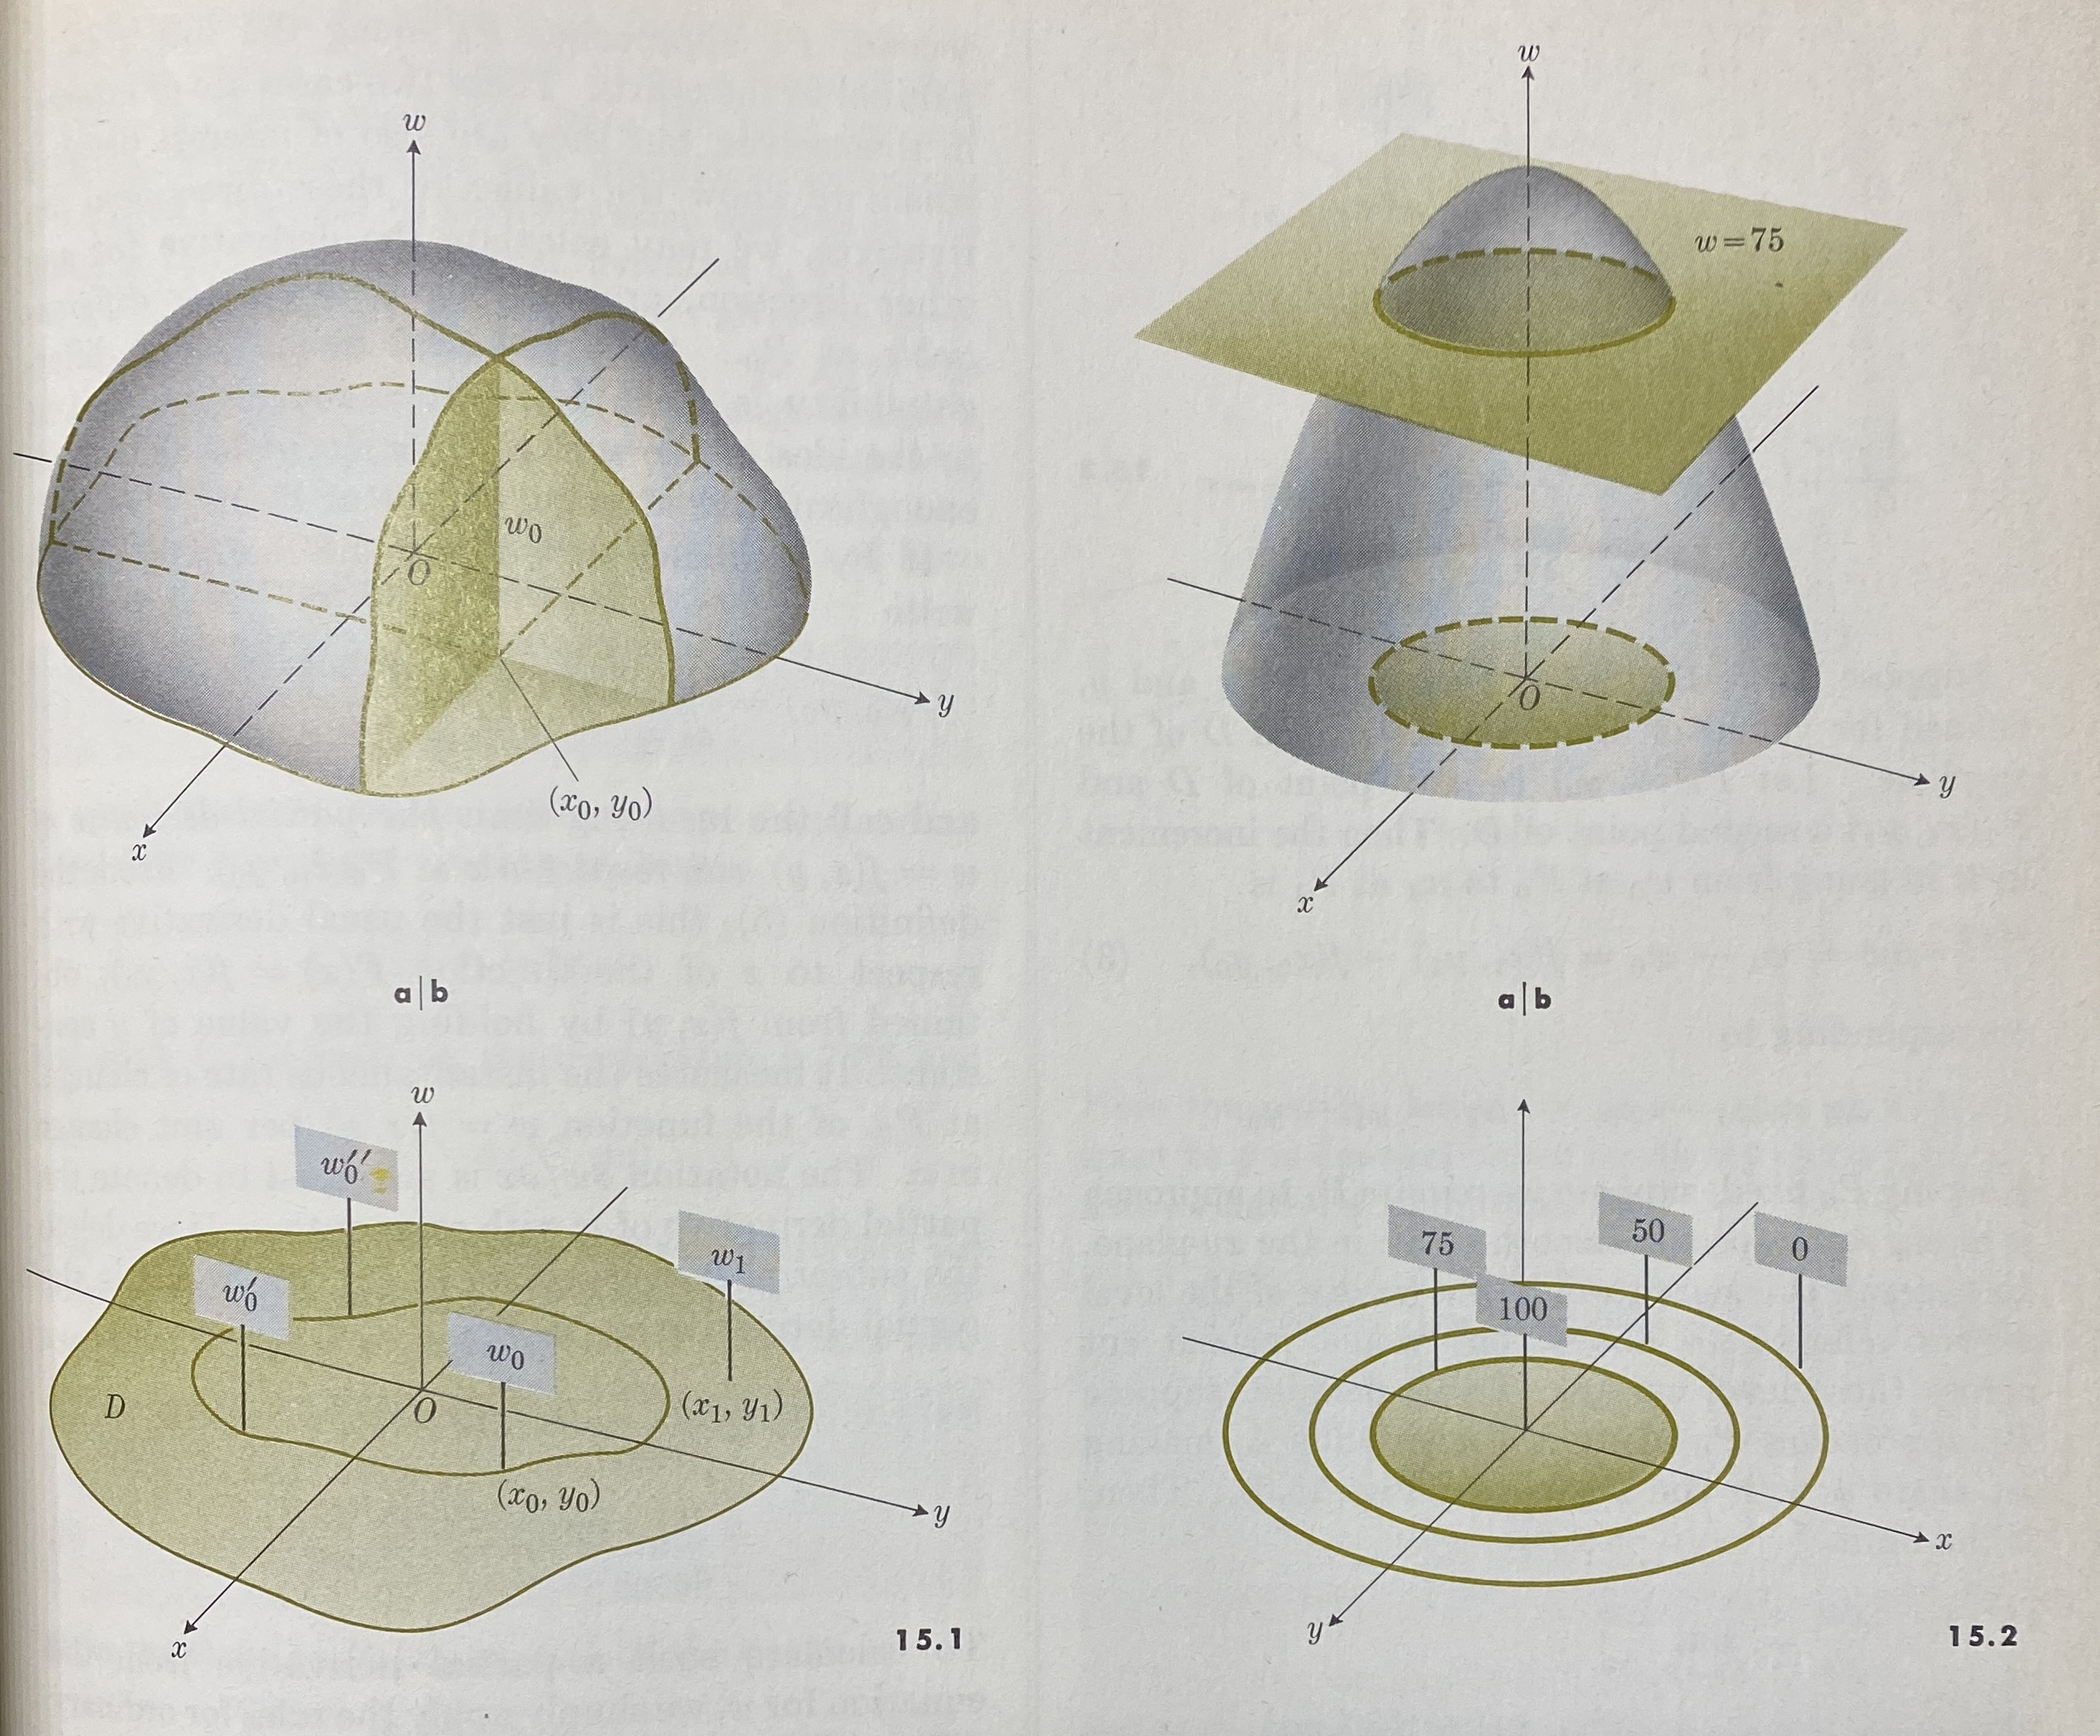
\includegraphics[width=0.7\linewidth]{ExtFiles/SurfacesAndContours.jpg}
    \caption{Surface plots and contour maps of 2D functions.}
    \label{fig:SurfacesAndContours}
\end{figure}
\begin{itemize}
    \item The equation $w=f(x,y)$ can be interpreted as representing a surface in $xyw$-space, or as a base region $D$ in the $xy$-plane with a marker bearing a corresponding $w$-value attached to each point.
    \begin{itemize}
        \item To introduce order into the second interpretation, we can construct a \textbf{contour map} with a number of \textbf{contour curves}.
    \end{itemize}
    \item \textbf{Contour curve}: A curve consisting of points $(x,y)\in D$ with equal $w$-values.
    \begin{itemize}
        \item The formula for such a curve can be derived by setting $w_0=f(x,y)$, where $w_0\in R_f$.
    \end{itemize}
    \item \textbf{Directional derivative} (of $f(x,y)$ at $(x_0,y_0)$ in the $\phi$-direction): The limit
    \begin{equation*}
        \dv{w}{s} = \lim_{\Delta s\to 0}\Dv{w}{s} = \lim_{P_1\to P_0}\frac{f(x_1,y_1)-f(x_0,y_0)}{\sqrt{\Delta x^2+\Delta y^2}}
    \end{equation*}
    \begin{figure}[h!]
        \centering
        \begin{tikzpicture}[
            every node/.append style={black}
        ]
            \footnotesize
            \draw [->] (-0.5,0) -- (5,0) node[right]{$x$};
            \draw [->] (0,-0.6) -- (0,4) node[above]{$y$};
            \node [anchor=north east] {$O$};

            \draw [ylx,thick] (0.4,0.3) coordinate (A) -- node[above]{$L$} (4.5,3.5) coordinate (B);
            \fill ($(A)!0.2!(B)$) coordinate (P0) circle (2pt) node[below right,xshift=-2mm]{$P_0(x_0,y_0)$};
            \fill ($(A)!0.8!(B)$) coordinate (P1) circle (2pt) node[right,yshift=-3pt]{$P_1(x_1,y_1)$};
            \begin{scope}[on background layer]
                \draw [ylx,semithick] (P0) -- node[pos=0.8,below]{$\Delta x$} (P0 -| P1) coordinate (R) -- node[right]{$\Delta y$} (P1);
            \end{scope}
            \pic [draw,->,angle radius=1cm,pic text={$\phi$},angle eccentricity=1.2] {angle=R--P0--P1};

            \node [fill=gay,minimum width=8mm] at ([yshift=1cm]P0) {$w_0$}
                edge [semithick] (P0)
            ;
            \node [fill=gay,minimum width=8mm] at ([yshift=1cm]P1) {$w_1$}
                edge [semithick] (P1)
            ;
        \end{tikzpicture}
        \caption{The directional derivative.}
        \label{fig:directionalDerivative}
    \end{figure}
    \begin{itemize}
        \item Basically, we let $P_1$ approach $P_0$ along a smooth curve (the line $L$ connecting $P_1$ and $P_0$ for simplicity and to be definite; $L$ makes an angle $\phi$ with the $x$-axis) and watch how $\Delta w=w_1-w_0=f(x_1,y_1)-f(x_0,y_0)$, $\Delta x=x_1-x_0$, and $\Delta y=y_1-y_0$ change.
        \item Note that the directional derivative does depend on the \emph{direction} from which $P_1$ approaches $P_0$, not just the absolute distance between $P_1$ and $P_0$.
    \end{itemize}
    \item We now consider two special cases: When \dq{$P_1$ approaches $P_0$ along the line $y=y_0$ parallel to the $x$-axis, [and when] $P_1$ approaches $P_0$ along the line $x=x_0$ parallel to the $y$-axis}{498}
    \begin{itemize}
        \item These cases are important because if $f(x,y)$ is \textbf{differentiable} at $P_0$, we can calculate the directional derivative in any direction from them.
    \end{itemize}
    \item \textbf{Partial derivative} (of $f(x,y)$ with respect to $x$ at $P_0(x_0,y_0)$): The value
    \begin{equation*}
        f_x(x_0,y_0) = \lim_{\Delta x\to 0}\frac{f(x_0+\Delta x,y_0)-f(x_0,y_0)}{\Delta x}
    \end{equation*}
    \begin{itemize}
        \item Essentially, this is the derivative with respect to $x$ of the function $g(x)=f(x,y)$ with $y$ held constant.
        \item It measures \dq{the instantaneous rate of change, at $P_0$, of the function [$f(x,y)$] per unit change in $x$}{498}
    \end{itemize}
    \item \textbf{Partial derivative} (of $w=f(x,y)$ with respect to $x$): The function
    \begin{equation*}
        \pdv{w}{x} = f_x(x,y) = \lim_{\Delta x\to 0}\frac{f(x+\Delta x,y)-f(x,y)}{\Delta x}
    \end{equation*}
    \begin{itemize}
        \item To evaluate this, we apply the ordinary rules of differentiation, treating $y$ as a constant. 
    \end{itemize}
    \item In either of the partial derivative definitions, $\Delta x$ can be positive or negative. However, if we take the directional derivative in the positive $x$ direction (for example), then $\Delta x$ in the partial derivative definitions can only be positive.
    \begin{itemize}
        \item Similarly, if $f_x$ exists, it gives the directional derivative in the positive $x$-direction, whereas $-f_x$ is the directional derivative in the negative $x$-direction.
    \end{itemize}
    \begin{figure}[h!]
        \centering
        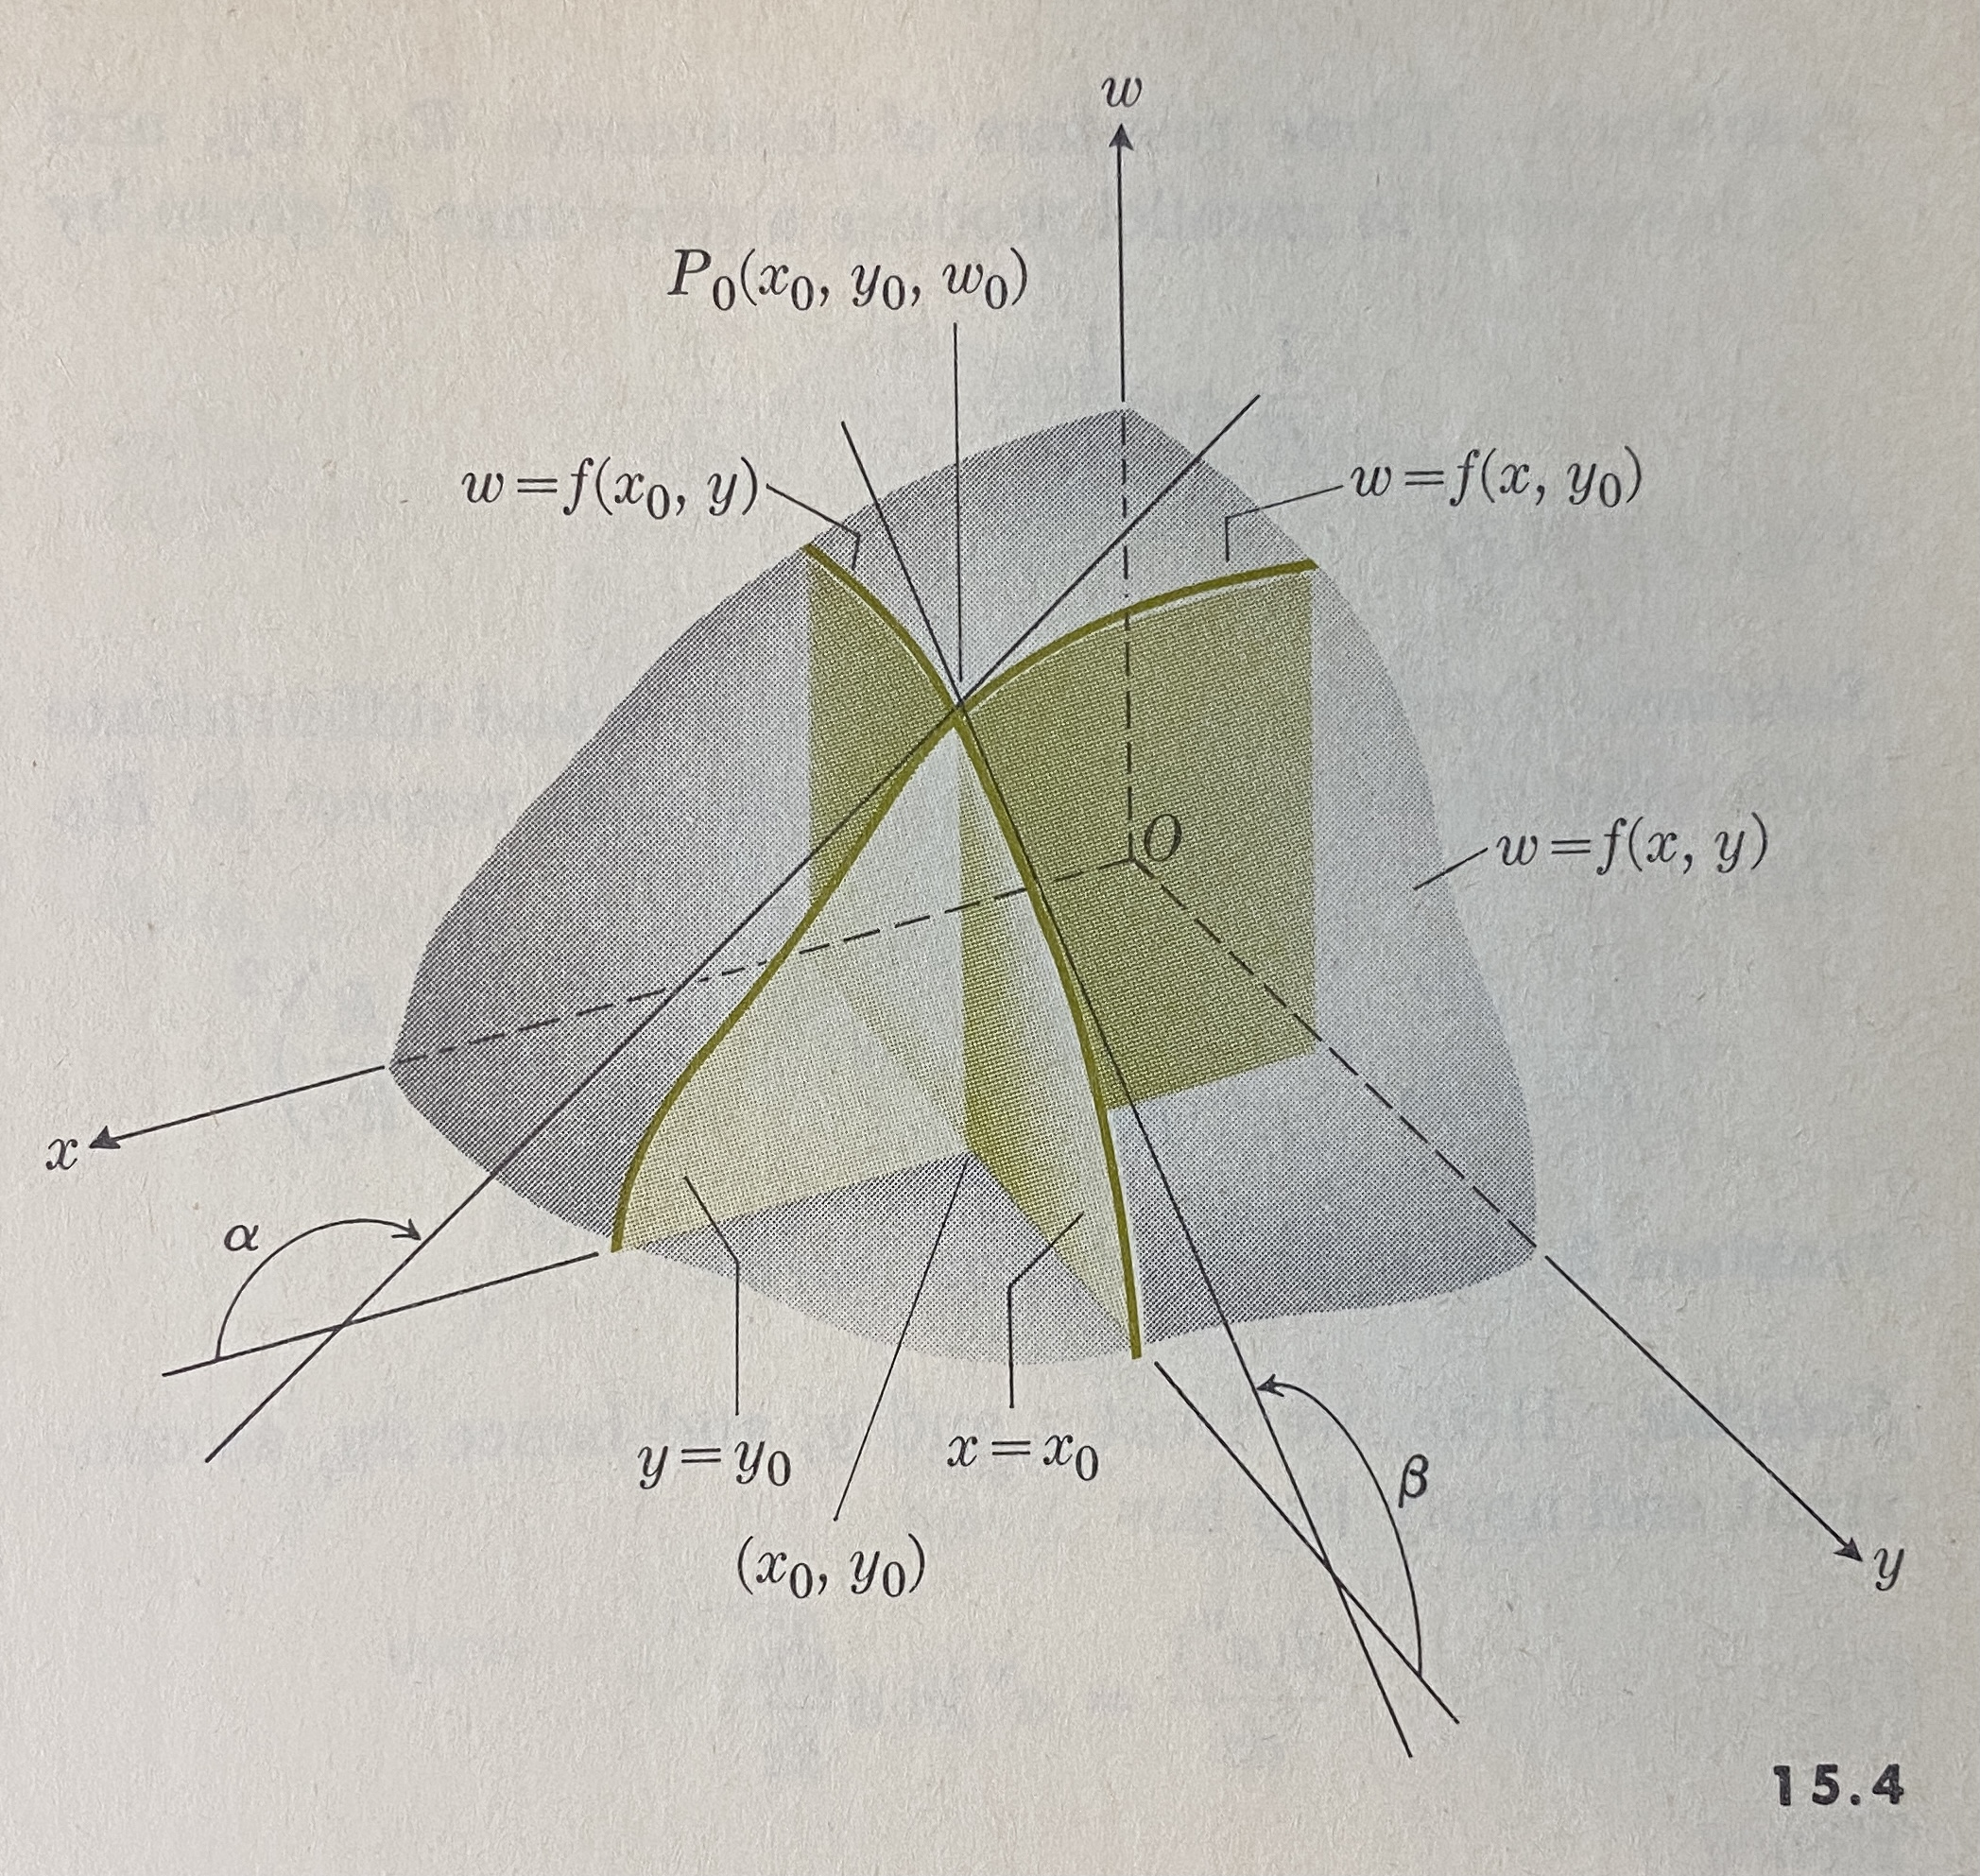
\includegraphics[width=0.4\linewidth]{ExtFiles/geometricPartialDv.jpg}
        \caption{Geometric interpretation of the partial derivative.}
        \label{fig:geometricPartialDv}
    \end{figure}
    \item As in Figure \ref{fig:geometricPartialDv}, the geometric interpretation of the partial derivative (wrt. $x$) at a point $P(x_0,y_0,w_0)$ is as the slope of the curve $f(x,y_0)$, and symetrically wrt. $y$.
    \item We can define the partial derivative with respect to $y$ similarly to how it is defined for $x$.
    \begin{equation*}
        \pdv{w}{y} = f_y(x,y) = \lim_{\Delta y\to 0}\frac{f(x,y+\Delta y)-f(x,y)}{\Delta y}
    \end{equation*}
    \item With higher order derivatives $\pdv*{w}{z}$, $\pdv*{w}{u}$, $\pdv*{w}{v}$, and more as in $w=f(x,y,z,u,v)$, we evaluate by holding all but the variable of interest constant.
    \item To denote the partial derivative at a point, we have two notations:
    \begin{align*}
        \left( \pdv{w}{x} \right)_{(x_0,y_0)}&&
            f_x(x_0,y_0)
    \end{align*}
\end{itemize}



\section{Tangent Plane and Normal Line}
\begin{itemize}
    \item \textbf{Tangent plane} (to $w=f(x,y)$ at $P_0(x_0,y_0,w_0)$): A plane $T$ such that for any point $P$ on the surface described by $f(x,y)$, as $P\to P_0$, the angle between $T$ and $\overline{PP_0}$ approaches 0.
    \item \textbf{Normal line} (to $w=f(x,y)$ at $P_0(x_0,y_0,w_0)$): The line through $P_0$ which is normal to the tangent plane to $f(x,y)$ at $P_0$.
    \item The tangent plane is determined by the lines $L_1$ and $L_2$ tangent to the curves $C_1:w=f(x_0,y)$ and $C_2:w=f(x,y_0)$; the slopes of these lines are given by $\pdv*{w}{y}$ and $\pdv*{w}{x}$, respectively.
    \item Formulae for the tangent plane and normal line follow easily after finding a normal vector $\vb{N}$ to the plane of $L_1$ and $L_2$. To find $\vb{N}$, we can use the cross product of the vectors $\vb{v}_1$ and $\vb{v}_2$ lying along $L_1$ and $L_2$, respectively.
    \begin{figure}[h!]
        \centering
        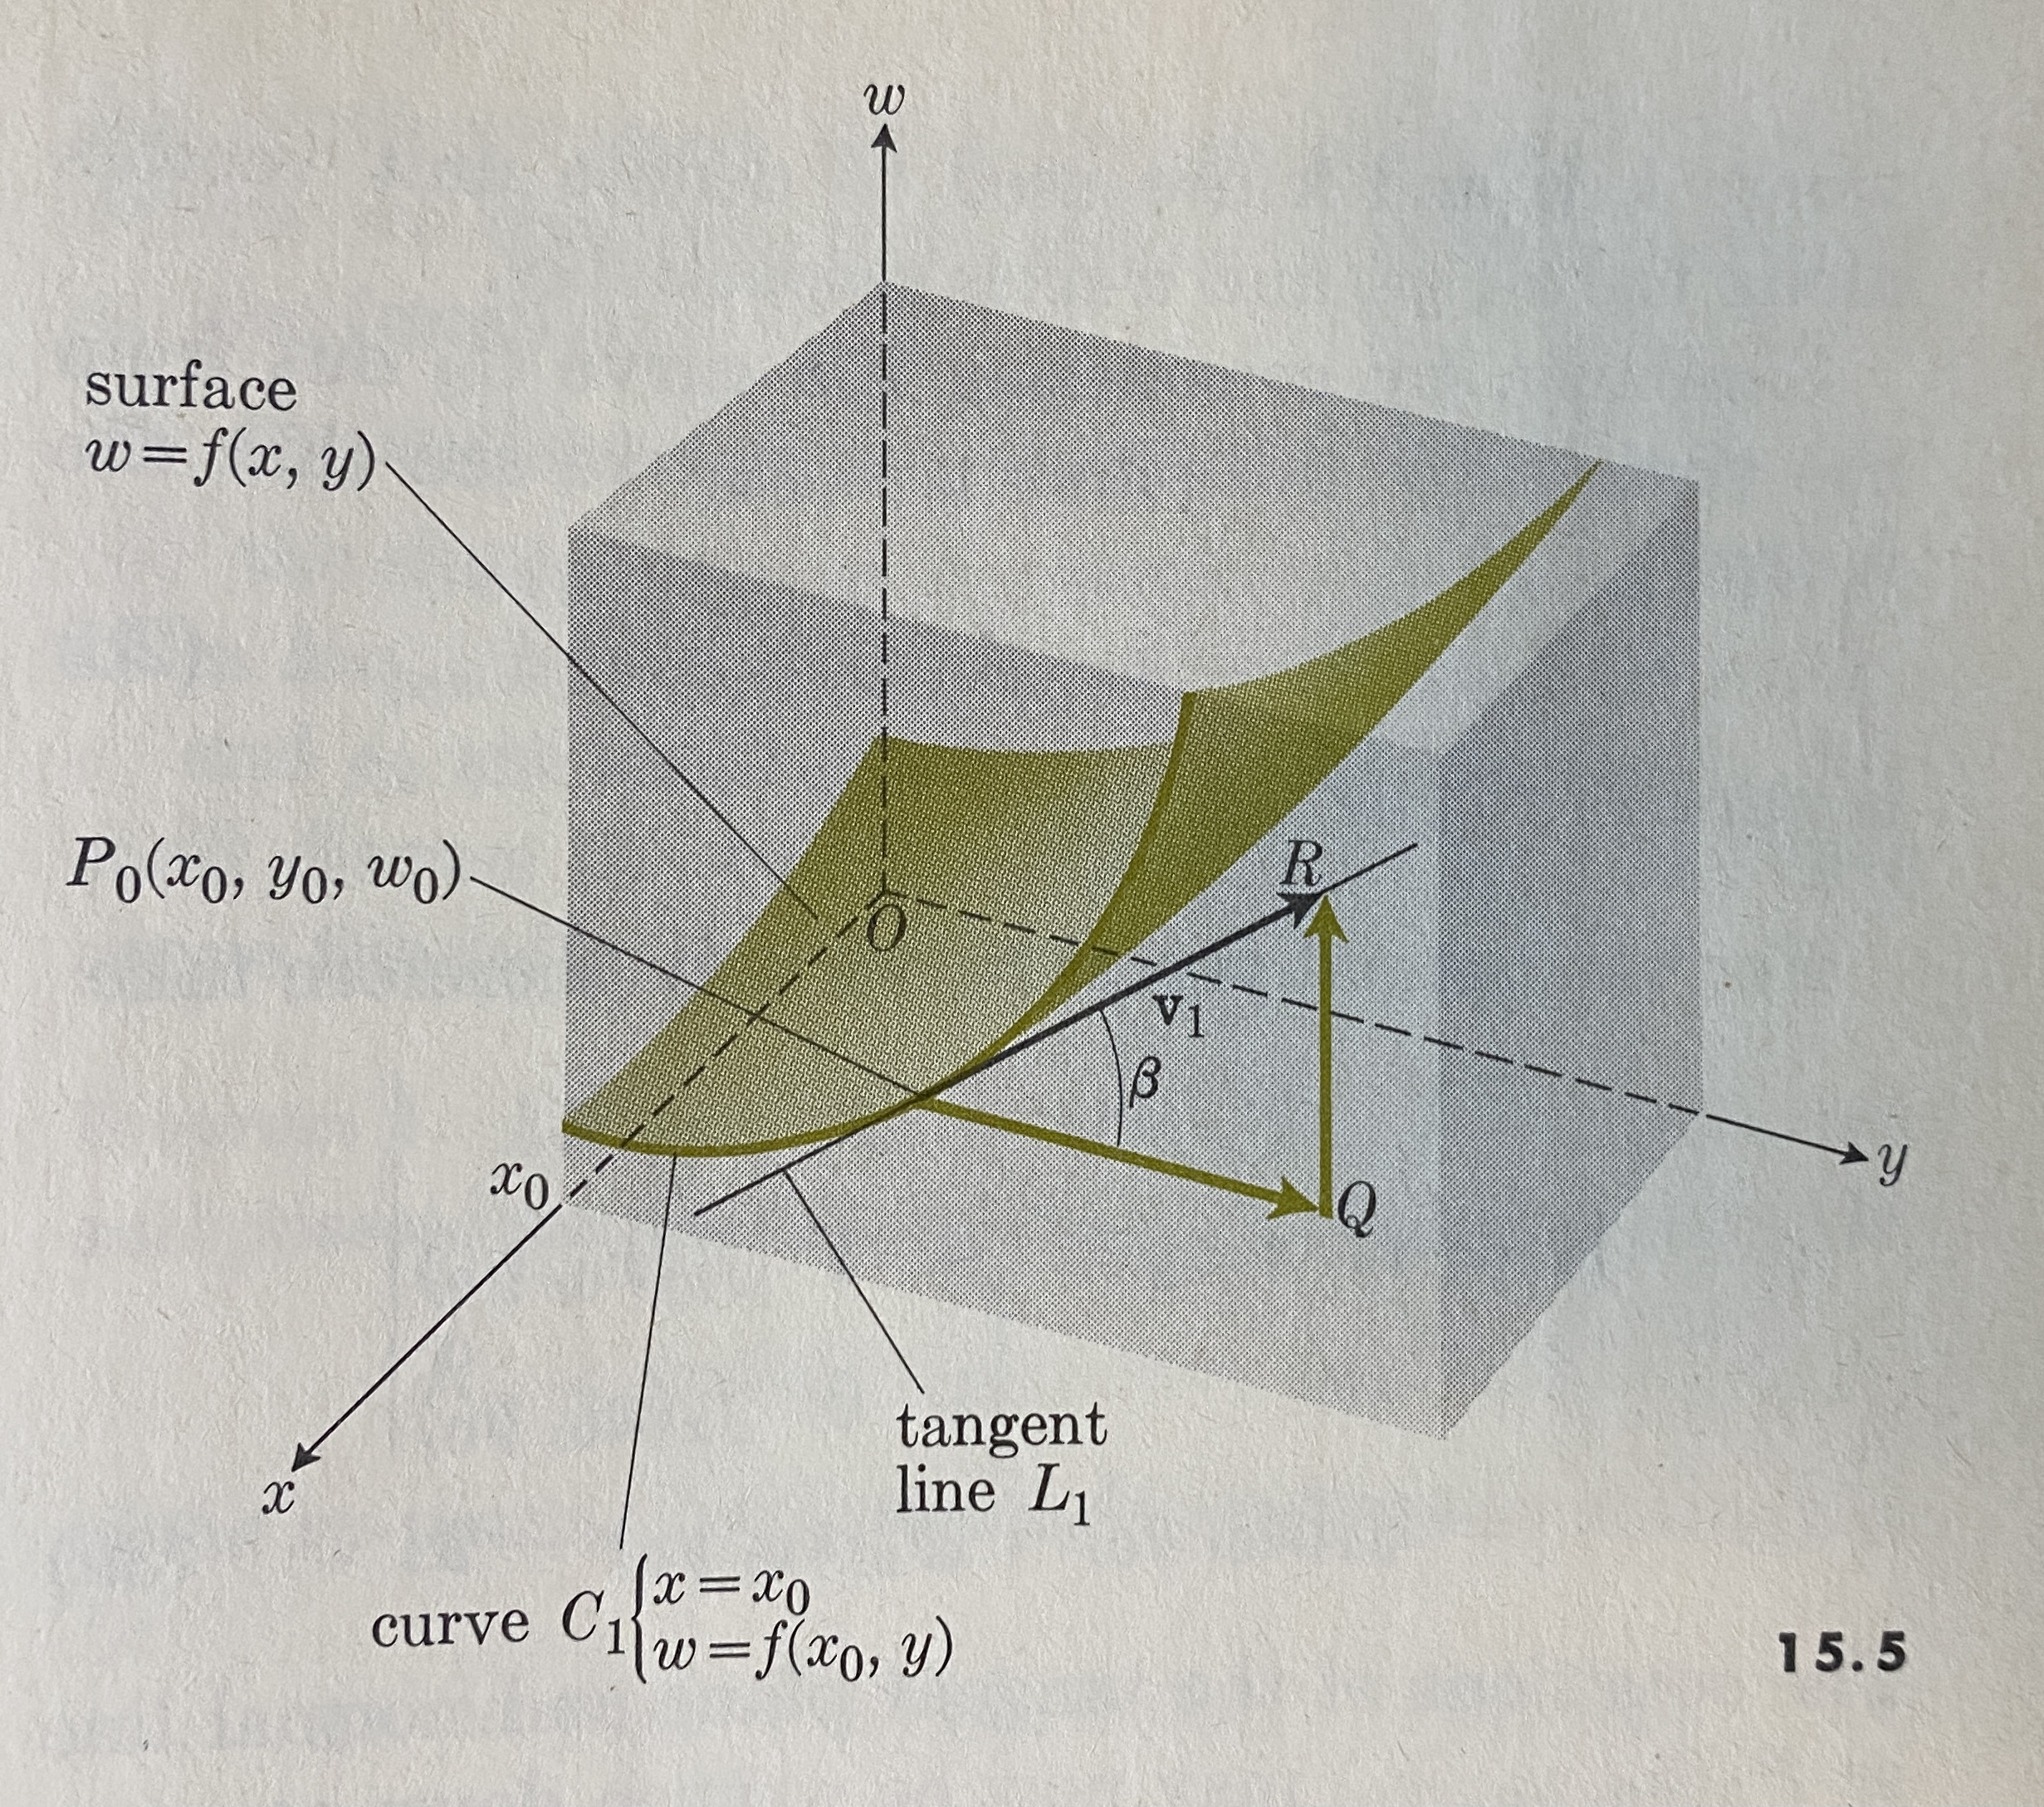
\includegraphics[width=0.4\linewidth]{ExtFiles/deriveTangentPlane.jpg}
        \caption{Deriving formulae for the tangent plane and normal line.}
        \label{fig:deriveTangentPlane}
    \end{figure}
    \begin{itemize}
        \item From Figure \ref{fig:deriveTangentPlane}, we can see that
        \begin{align*}
            \vb{v}_1 &= \vb{j}+f_y(x_0,y_0)\vb{k}&
                \vb{v}_2 &= \vb{i}+f_x(x_0,y_0)\vb{k}
        \end{align*}
        \item Thus,
        \begin{equation*}
            \vb{N} = \vb{i}f_x(x_0,y_0)+\vb{j}f_y(x_0,y_0)-\vb{k}
        \end{equation*}
        \item Therefore, the formulae for the tangent plane and normal line, respectively, are
        \begin{align*}
            A(x-x_0)+B(y-y_0)+C(w-w_0) &= 0&
                (x,y,w) &= (x_0,y_0,w_0)+t(A,B,C)
        \end{align*}
        where $A=f_x(x_0,y_0)$, $B=f_y(x_0,y_0)$, $C=-1$, and $t\in(-\infty,\infty)$.
        \item In vector form, if $\vb{R}=\vb{i}x+\vb{j}y+\vb{k}z$ and $\vb{R}_0=\vb{i}x_0+\vb{j}y_0+\vb{k}z_0$, then
        \begin{align*}
            \vb{N} &= \vb{i}f_x(x_0,y_0)+\vb{j}f_y(x_0,y_0)-\vb{k}&
                \vb{N}\cdot(\vb{R}-\vb{R}_0) &= 0&
                    \vb{R} &= \vb{R}_0+t\vb{N}
        \end{align*}
    \end{itemize}
\end{itemize}



\section{Approximate Value of \texorpdfstring{$\Delta w$}{TEXT}}
\begin{itemize}
    \item \textbf{Linearization} (of $f$ at $P_0$): The function (based off of the tangent plane)
    \begin{equation*}
        w = f(x_0,y_0)+f_x(x_0,y_0)\cdot(x-x_0)+f_y(x_0,y_0)\cdot(y-y_0)
    \end{equation*}
    \item Note that
    \begin{equation*}
        \Delta w_\text{tan} = f_x(x_0,y_0)\Delta x+f_y(x_0,y_0)\Delta y
    \end{equation*}
    meaning that to calculate $\Delta w_\text{tan}$, we need only add the tangential components; no other interaction term is needed.
    \item Important results:
    \begin{thm}\label{thm:deltaW}
        Let the function $w=f(x,y)$ be continuous and possess partial derivatives $f_x,f_y$ throughout a region $R:|x-x_0|<h,\ |y-y_0|<k$ of the $xy$-plane. Let $f_x$ and $f_y$ be continuous at $(x_0,y_0)$. Let $\Delta w = f(x_0+\Delta x,y_0+\Delta y)-f(x_0,y_0)$. Then
        \begin{equation*}
            \Delta w = f_x(x_0,y_0)\Delta x+f_y(x_0,y_0)\Delta y+\epsilon_1\Delta x+\epsilon_2\Delta y
        \end{equation*}
        where $\epsilon_1,\epsilon_2\to 0$ when $\Delta x,\Delta y\to 0$.
    \end{thm}
    \begin{cly}
        Let $w=f(x,y)$ be continuous in a region $R:|x-x_0|<h,\ |y-y_0|<k$. Let $f_x$ and $f_y$ exist in $R$ and be continuous at $(x_0,y_0)$. Then the surface $w=f(x,y)$ has a tangent plane at $P_0(x_0,y_0,w_0)$, where $w_0=f(x_0,y_0)$.
    \end{cly}
    \begin{itemize}
        \item These results extend into finitely higher dimensions.
    \end{itemize}
\end{itemize}



\section{The Directional Derivative: General Case}
\begin{itemize}
    \item \marginnote{12/17:}We first prove that the directional derivative can be expressed in terms of the partial derivatives.
    \begin{thm}
        Let $w=f(x,y)$ be continuous and possess partial derivatives $f_x$, $f_y$ throughout some neighborhood of the point $P_0(x_0,y_0)$. Let $f_x$ and $f_y$ be continuous at $P_0$. Then the directional derivative at $P_0$ exists for any direction angle $\phi$ and is given by
        \begin{equation*}
            \dv{w}{s} = f_x(x_0,y_0)\cos\phi+f_y(x_0,y_0)\sin\phi
        \end{equation*}
        \begin{proof}
            By Theorem \ref{thm:deltaW}, we know that $\Delta w=f_x(x_0,y_0)\Delta x+f_y(x_0,y_0)\Delta y+\epsilon_1\Delta x+\epsilon_2\Delta y$ where $\epsilon_1,\epsilon_2\to 0$ as $\Delta x,\Delta y\to 0$. Thus,
            \begin{equation*}
                \Dv{w}{s} = f_x(x_0,y_0)\Dv{x}{s}+f_y(x_0,y_0)\Dv{y}{s}+\epsilon_1\Dv{x}{s}+\epsilon_2\Dv{y}{s}
            \end{equation*}
            where $\epsilon_1,\epsilon_2\to 0$ as $\Delta x,\Delta y\to 0$. Hence, since $\lim\Dv{w}{s}=\dv{w}{s}$, $\lim\Dv{x}{s}=\dv{x}{s}=\cos\phi$, and $\lim\Dv{y}{s}=\dv{y}{s}=\sin\phi$, we have
            \begin{equation*}
                \dv{w}{s} = f_x(x_0,y_0)\cos\phi+f_y(x_0,y_0)\sin\phi
            \end{equation*}
            as desired.
        \end{proof}
    \end{thm}
    \begin{itemize}
        \item Note that $\phi=0,\frac{\pi}{2},\pi,\frac{3\pi}{2}$ lead to $\dv*{w}{s}=\pdv*{w}{x},\pdv*{w}{y},-\pdv*{w}{x},-\pdv*{w}{y}$, respectively.
    \end{itemize}
    \item The directional derivative in three dimensions is given by
    \begin{equation*}
        \dv{w}{s} = f_x(x_0,y_0,z_0)\cos\alpha+f_y(x_0,y_0,z_0)\cos\beta+f_z(x_0,y_0,z_0)\cos\gamma
    \end{equation*}
    \begin{itemize}
        \item If we have a direction vector $\vb{u}=\vb{i}\cos\alpha+\vb{j}\cos\beta+\vb{k}\cos\gamma$ and another one that depends on the function and $P_0$ (the \textbf{gradient}) given by $\vb{v}=\vb{i}f_x(x_0,y_0,z_0)+\vb{j}f_y(x_0,y_0,z_0)+\vb{k}f_z(x_0,y_0,z_0)$, then
    \end{itemize}
    \begin{equation*}
        \dv{w}{s} = \vb{u}\cdot\vb{v}
    \end{equation*}
\end{itemize}



\section{The Gradient}
\begin{itemize}
    \item \textbf{Gradient} (of $w$): The vector function
    \begin{equation*}
        \gradd w = \nabla w = \vb{i}\pdv{w}{x}+\vb{j}\pdv{w}{y}+\vb{k}\pdv{w}{z}
    \end{equation*}
    \item The inverted capital delta is the \textbf{del operator}. In its own right, it is defined by
    \begin{equation*}
        \nabla = \vb{i}\pdv{x}+\vb{j}\pdv{y}+\vb{k}\pdv{z}
    \end{equation*}
    \item Recall that the directional derivative at $P_0(x_0,y_0,z_0)$ can be written as
    \begin{equation*}
        \left( \dv{w}{s} \right)_0 = (\nabla w)_0\cdot\vb{u}
    \end{equation*}
    \begin{itemize}
        \item The significance of this is that it implies that
        \begin{equation*}
            \left( \dv{w}{s} \right)_0 = |(\nabla w)_0|\, |u|\, \cos\theta = |(\nabla w)_0|\, \cos\theta
        \end{equation*}
        which means that the directional derivative is the \dq{scalar projection of $\gradd w$ at $P_0$, onto the direction $\vb{u}$}{511}
        \item Since $\dv*{w}{s}$ is maximized when $\cos\theta=1$, it must be that \dq{the function $w=f(x,y,z)$ changes most rapidly in the direction given by the vector $\gradd w$ itself. Moreover, the directional derivative in this direction is equal to the magnitude of the gradient}{511}
    \end{itemize}
    \item The gradient vector at $P_0(x_0,y_0,z_0)$, where $w_0=f(x_0,y_0,z_0)$ is also normal to the contour surface consisting of all points $P(x,y,z)$ for which $f(x,y,z)=w_0$.
    \begin{itemize}
        \item We can prove this from the fact that the directional derivative in the direction of any line tangent to $P_0$ along the contour surface will be 0. But since $(\nabla w)_0\neq\vb{0}$, we must have $\cos\theta=0$, meaning that $\nabla w$ is perpendicular to any line tangent to $P_0$. It follows that it is normal to the contour surface, itself.
    \end{itemize}
    \item Be careful with dimensions: The 3D vector $\gradd w$ is points in the direction in 3-space of greatest change for a function with a 3D domain (a function best graphed in 4D), but is normal to a 2D surface that is a subset of this 3D domain.
\end{itemize}



\section{The Chain Rule for Partial Derivatives}
\begin{itemize}
    \item Let $w=f(x,y,z)$ be a function with continuous partial derivatives $f_x,f_y,f_z$ throughout some region $R$ of $xyz$-space. If $C$ is a curve lying in $R$ defined by the parameterization $x=x(t)$, $y=y(t)$, and $z=z(t)$, then
    \begin{equation*}
        \dv{w}{t} = \pdv{w}{x}\dv{x}{t}+\pdv{w}{y}\dv{y}{t}+\pdv{w}{z}\dv{z}{t}
    \end{equation*}
    \begin{itemize}
        \item By generalizing Theorem \ref{thm:deltaW} to three dimensions and dividing by $\Delta t$, we have
        \begin{equation*}
            \Dv{w}{t} = \left( \pdv{w}{x} \right)_0\Dv{x}{t}+\left( \pdv{w}{t} \right)_0\Dv{y}{t}+\left( \pdv{w}{z} \right)_0\Dv{z}{t}+\epsilon_1\Dv{x}{t}+\epsilon_2\Dv{y}{t}+\epsilon_3\Dv{z}{t}
        \end{equation*}
        where $\epsilon_1,\epsilon_2,\epsilon_3\to 0$ as $\Delta x,\Delta y,\Delta z\to 0$.
        \item Now if $C$ is differentiable in $R$, too, (i.e., $\dv*{x}{t},\dv*{y}{t},\dv*{z}{t}$ all exist) then $\Delta x,\Delta y,\Delta z\to 0$ as $\Delta t\to 0$.
        \item Therefore, if we take the limit as $\Delta t\to 0$ of the above equation, we get the desired result.
    \end{itemize}
    \item Note that we can also write
    \begin{equation*}
        \dv{w}{t} = \nabla w\cdot\vb{v}
    \end{equation*}
    where $\vb{v}$ is the velocity vector along the curve $C$.
    \item We can also consider the behavior of a function along a surface $S$ lying in $R$ parameterized by $x=x(r,s)$, $y=y(r,s)$, and $z=z(r,s)$. In this case we can take
    \begin{align*}
        \pdv{w}{r} &= \pdv{w}{x}\pdv{x}{r}+\pdv{w}{y}\pdv{y}{r}+\pdv{w}{z}\pdv{z}{r}&
            \pdv{w}{s} &= \pdv{w}{x}\pdv{x}{s}+\pdv{w}{y}\pdv{y}{s}+\pdv{w}{z}\pdv{z}{s}
    \end{align*}
    \begin{itemize}
        \item We can also expand this to many more dimensions. This idea is best summarized in matrix form (for a function $w=f(x_1,\dots,x_n)$ parameterized by $x_1=x_1(y_1,\dots,y_m)$, \dots, $x_n=(y_1,\dots,y_m)$):
        \begin{equation*}
            \renewcommand{\arraystretch}{1.6}
            \begin{bmatrix}
                \pdv{w}{y_1} & \pdv{w}{y_2} & \cdots & \pdv{w}{y_m}\\
            \end{bmatrix}
            =
            \begin{bmatrix}
                \pdv{w}{x_1} & \pdv{w}{x_2} & \cdots & \pdv{w}{x_n}\\
            \end{bmatrix}
            \begin{bmatrix}
                \pdv{x_1}{y_1} & \pdv{x_1}{y_2} & \cdots & \pdv{x_1}{y_m}\\
                \pdv{x_2}{y_1} & \pdv{x_2}{y_2} & \cdots & \pdv{x_2}{y_m}\\
                \vdots         & \vdots         & \ddots & \vdots        \\
                \pdv{x_n}{y_1} & \pdv{x_n}{y_2} & \cdots & \pdv{x_n}{y_m}\\
            \end{bmatrix}
        \end{equation*}
    \end{itemize}
    \item To clarify the above results, we investigate a few problems.
    \item \dq{Suppose that $w=r^2\cos2\theta$, where $x=r\cos\theta$, $y=r\sin\theta$, $r=\sqrt{x^2+y^2}$, [and] $\theta=\tan^{-1}(y/x)$. Find $\pdv*{w}{x}$ and $\pdv*{w}{y}$}{516}
    \begin{itemize}
        \item We use the matrix methods to get an equation for the desired results.
        \renewcommand{\arraystretch}{1.6}
        \begin{align*}
            \begin{bmatrix}
                \pdv{w}{x} & \pdv{w}{y}\\
            \end{bmatrix}
            &=
            \begin{bmatrix}
                \pdv{w}{r} & \pdv{w}{\theta}\\
            \end{bmatrix}
            \begin{bmatrix}
                \pdv{r}{x} & \pdv{r}{y}\\
                \pdv{\theta}{x} & \pdv{\theta}{y}\\
            \end{bmatrix}\\
            &=
            \begin{bmatrix}
                2r\cos 2\theta & -2r^2\sin 2\theta\\
            \end{bmatrix}
            \begin{bmatrix}
                \frac{x}{r} & \frac{y}{r}\\
                -\frac{y}{r^2} & \frac{x}{r^2}\\
            \end{bmatrix}\\
            &=
            \begin{bmatrix}
                2x\cos 2\theta+2y\sin 2\theta & 2y\cos2\theta-2x\sin 2\theta
            \end{bmatrix}
        \end{align*}
        \item Now, we can use some substitutions to put the above results in terms of the variable with respect to which we are differentiating.
        \begin{align*}
            \pdv{w}{x} &= 2(x\cos 2\theta+y\sin 2\theta)&
                \pdv{w}{y} &= 2(y\cos 2\theta-x\sin 2\theta)\\
            &= 2r(\cos\theta\cos 2\theta+\sin\theta\sin 2\theta)&
                &= 2r(\sin\theta\cos 2\theta-\cos\theta\sin 2\theta)\\
            &= 2r\cos(2\theta-\theta)&
                &= 2r\sin(\theta-2\theta)\\
            &= 2x&
                &= -2y
        \end{align*}
    \end{itemize}
    \item \dq{Show that the change of variables from $x$ and $y$ to $r=y-ax$ [and] $s=y+ax$ transforms the differential equation $$\pdv{w}{x}-a\pdv{w}{y}=0$$ into a form that is more easily solved, and solve it. (Here $a$ is a constant.)}{516}
    \begin{itemize}
        \item We divide into two cases ($a\neq 0$ and $a=0$), beginning with the former.
        \item Imagine that $w=f(x,y)$ is transformed into $w=\tilde{f}(r,s)$ via substitutions which can be derived by treating the definitions of $r$ and $s$ as a two-variable system of equations and solving for $x$ and $y$.
        \begin{align*}
            x &= \frac{1}{2a}(s-r)&
                y &= \frac{1}{2}(r+s)
        \end{align*}
        \item Now to find $\pdv*{w}{x}$ and $\pdv*{w}{y}$, we use the chain rule.
        \begin{align*}
            \begin{bmatrix}
                \pdv{w}{x} & \pdv{w}{y}\\
            \end{bmatrix}
            &=
            \begin{bmatrix}
                \pdv{w}{r} & \pdv{w}{s}\\
            \end{bmatrix}
            \renewcommand{\arraystretch}{1.6}
            \begin{bmatrix}
                \pdv{r}{x} & \pdv{r}{y}\\
                \pdv{s}{x} & \pdv{s}{y}\\
            \end{bmatrix}\\
            &=
            \begin{bmatrix}
                \pdv{w}{r} & \pdv{w}{s}\\
            \end{bmatrix}
            \begin{bmatrix}
                -a & 1\\
                a & 1\\
            \end{bmatrix}\\
            &=
            \begin{bmatrix}
                -a\pdv{w}{r}+a\pdv{w}{s} & \pdv{w}{r}+\pdv{w}{s}
            \end{bmatrix}
        \end{align*}
        \item By substituting into the original differential equation, we get $-2a\pdv*{w}{r}=0$, or $\pdv{w}{r}=0$.
        \item Thus, this differential equation is easy to solve --- we need only require that $w$ is constant in the $r$-direction. Indeed, $w$ can be any function of $s$. Therefore, the solution is
        \begin{equation*}
            w = \phi(s) = \phi(y+ax)
        \end{equation*}
        where $\phi(s)$ is any differentiable function of $s$, whatsoever.
        \item If $a=0$, then we have the similar case $\pdv*{w}{x}=0$.
        \item Note that in solving an ordinary differential equation, we often get constants of integration. In solving a partial differentiable equation, arbitrary functions (such as $\phi(s)$) are analogous to these constants of integration. Extending the analogy, they can sometimes be solved for with "initial conditions," as in the next problem.
    \end{itemize}
    \item Find an explicit formula for $w$ in the above problem if its values along the $x$-axis are given by $w=\sin x$ and if $a\neq 0$.
    \begin{itemize}
        \item The general solution is $w=f(x,y)=\phi(y+ax)$.
        \item We are given $f(x,0)=\phi(0+ax)=\sin x$.
        \item Thus, if we let $u=ax$, we have $\phi(u)=\sin\frac{u}{a}$, meaning that $w=\phi(y+ax)=\sin\frac{y+ax}{a}$.
    \end{itemize}
\end{itemize}



\section{The Total Differential}
\begin{itemize}
    \item \textbf{Partial differential} (of $w=f(x,y,z)$ with respect to $x$): The infinitesimal value
    \begin{equation*}
        \pdv{w}{x}\dd{x}
    \end{equation*}
    \begin{itemize}
        \item There also exist symmetric partial differentials with respect to $y$ and $z$.
    \end{itemize}
    \item \textbf{Total differential} (of $w=f(x,y,z)$): The infinitesimal value
    \begin{equation*}
        \dd{w} = \pdv{w}{x}\dd{x}+\pdv{w}{y}\dd{y}+\pdv{w}{z}\dd{z}
    \end{equation*}
    that is the sum of the partial differentials of $w$.
    \item If $x,y,z$ are given as functions of a single variable $t$, we have
    \begin{align*}
        \dd{x} &= x'(t)\dd{t}&
            \dd{y} &= y'(t)\dd{t}&
                \dd{z} &= z'(t)\dd{t}
    \end{align*}
    \item If $x,y,z$ are given as functions of two variables $r,s$, their total differentials are
    \begin{align*}
        \dd{x} &= \pdv{x}{r}\dd{r}+\pdv{x}{s}\dd{s}&
            \dd{y} &= \pdv{y}{r}\dd{r}+\pdv{y}{s}\dd{s}&
                \dd{z} &= \pdv{z}{r}\dd{r}+\pdv{z}{s}\dd{s}
    \end{align*}
    \begin{itemize}
        \item If we take the perspective that $w=f[x(r,s),y(r,s),z(r,s)]=\tilde{f}(r,s)$ is a function of two variables, then we should have
        \begin{equation*}
            \dd{w} = \pdv{w}{r}\dd{r}+\pdv{w}{s}\dd{s}
        \end{equation*}
        \item Now this $\dd{w}$ is the same as the one given earlier with respect to $x,y,z$, as a consequence of the chain rule. Indeed,
        \begin{align*}
            \dd{w} &= \pdv{w}{x}\left( \pdv{x}{r}\dd{r}+\pdv{x}{s}\dd{s} \right)+\pdv{w}{y}\left( \pdv{y}{r}\dd{r}+\pdv{y}{s}\dd{s} \right)+\pdv{w}{z}\left( \pdv{z}{r}\dd{r}+\pdv{z}{s}\dd{s} \right)\\
            &= \left( \pdv{w}{x}\pdv{x}{r}+\pdv{w}{y}\pdv{y}{r}+\pdv{w}{z}\pdv{z}{r} \right)\dd{r}+\left( \pdv{w}{x}\pdv{x}{s}+\pdv{w}{y}\pdv{y}{s}+\pdv{w}{z}\pdv{z}{s} \right)\dd{s}\\
            &= \pdv{w}{r}\dd{r}+\pdv{w}{s}\dd{s}
        \end{align*}
        \item Note that $r$ and $s$ are the independent variables here, so while we can approximate $\dd{r}$ and $\dd{s}$ with $\Delta r$ and $\Delta s$, respectively, we should not approximate $\dd{x},\dd{y},\dd{z}$ with $\Delta x,\Delta y,\Delta z$. Indeed, we should use the differentials $\dd{x},\dd{y},\dd{z}$ as defined in terms of $\dd{r},\dd{s}$ to approximate $\Delta x,\Delta y,\Delta z$.
    \end{itemize}
    \item These results can be generalized to higher dimensions.
    \item The following example should make clear the power of these differential definitions: \dq{Consider the function $w=x^2+y^2+z^2$ with $x=r\cos s$, $y=r\sin s$, [and] $z=r$}{519}
    \begin{itemize}
        \item The total differential is $\dd{w}=2(x\dd{x}+y\dd{y}+z\dd{z})$.
        \item The differentials in terms of $r$ and $s$ are $\dd{x}=\cos s\dd{r}-r\sin s\dd{s}$, $\dd{y}=\sin s\dd{r}+r\cos s\dd{s}$, and $\dd{z}=\dd{r}$.
        \item Hence, the total differential can also be written as
        \begin{align*}
            \dd{w} &= 2(x\cos s+y\sin s+z)\dd{r}+2(-xr\sin s+yr\cos s)\dd{s}\\
            &= 2(r\cos^2s+r\sin^2s+r)\dd{r}+2(-r^2\cos s\sin s+r^2\sin s\cos s)\dd{s}\\
            &= 4r\dd{r}
        \end{align*}
        \item Integrating, the above yields $w=2r^2$.
        \item Critically, we can also derive this formula for $w$ from the original function and parameterization since $w=r^2\cos^2s+r^2\sin^2s+r^2=2r^2$.
    \end{itemize}
    \item If $F(x,y)=0$, then for the plane curve generated, $\dv*{y}{x}=-F_x(x,y)/F_y(x,y)$ if $F_y(x,y)\neq 0$.
    \begin{itemize}
        \item We can also derive this result by implicitly differentiating $F(x,y)=0$, as we are allowed to by the \textbf{implicit function theorem}.
    \end{itemize}
\end{itemize}



\section{Maxima and Minima of Functions of Two Independent Variables}
\begin{itemize}
    \item \marginnote{12/18:}\textbf{Relative minimum} (of $f(x,y)$): A point $(a,b)$, in a region $R$ where $f$ is defined, continuous, and has continuous partial derivatives with respect to $x$ and $y$, such that $f(x,y)\geq f(a,b)$ for all points $(x,y)$ sufficiently close to $(a,b)$. \emph{Also known as} \textbf{local minimum}.
    \item \textbf{Relative maximum} (of $f(x,y)$): A point $(a,b)$, in a region $R$ where $f$ is defined, continuous, and has continuous partial derivatives with respect to $x$ and $y$, such that $f(x,y)\leq f(a,b)$ for all points $(x,y)$ sufficiently close to $(a,b)$. \emph{Also known as} \textbf{local maximum}.
    \item \textbf{Absolute minimum} (of $f(x,y)$): A relative minimum $(a,b)$ of $f(x,y)$ such that $f(x,y)\geq f(a,b)$ for all $(x,y)\in R$.
    \item \textbf{Absolute maximum} (of $f(x,y)$): A relative maximum $(a,b)$ of $f(x,y)$ such that $f(x,y)\leq f(a,b)$ for all $(x,y)\in R$.
    \begin{figure}[h!]
        \centering
        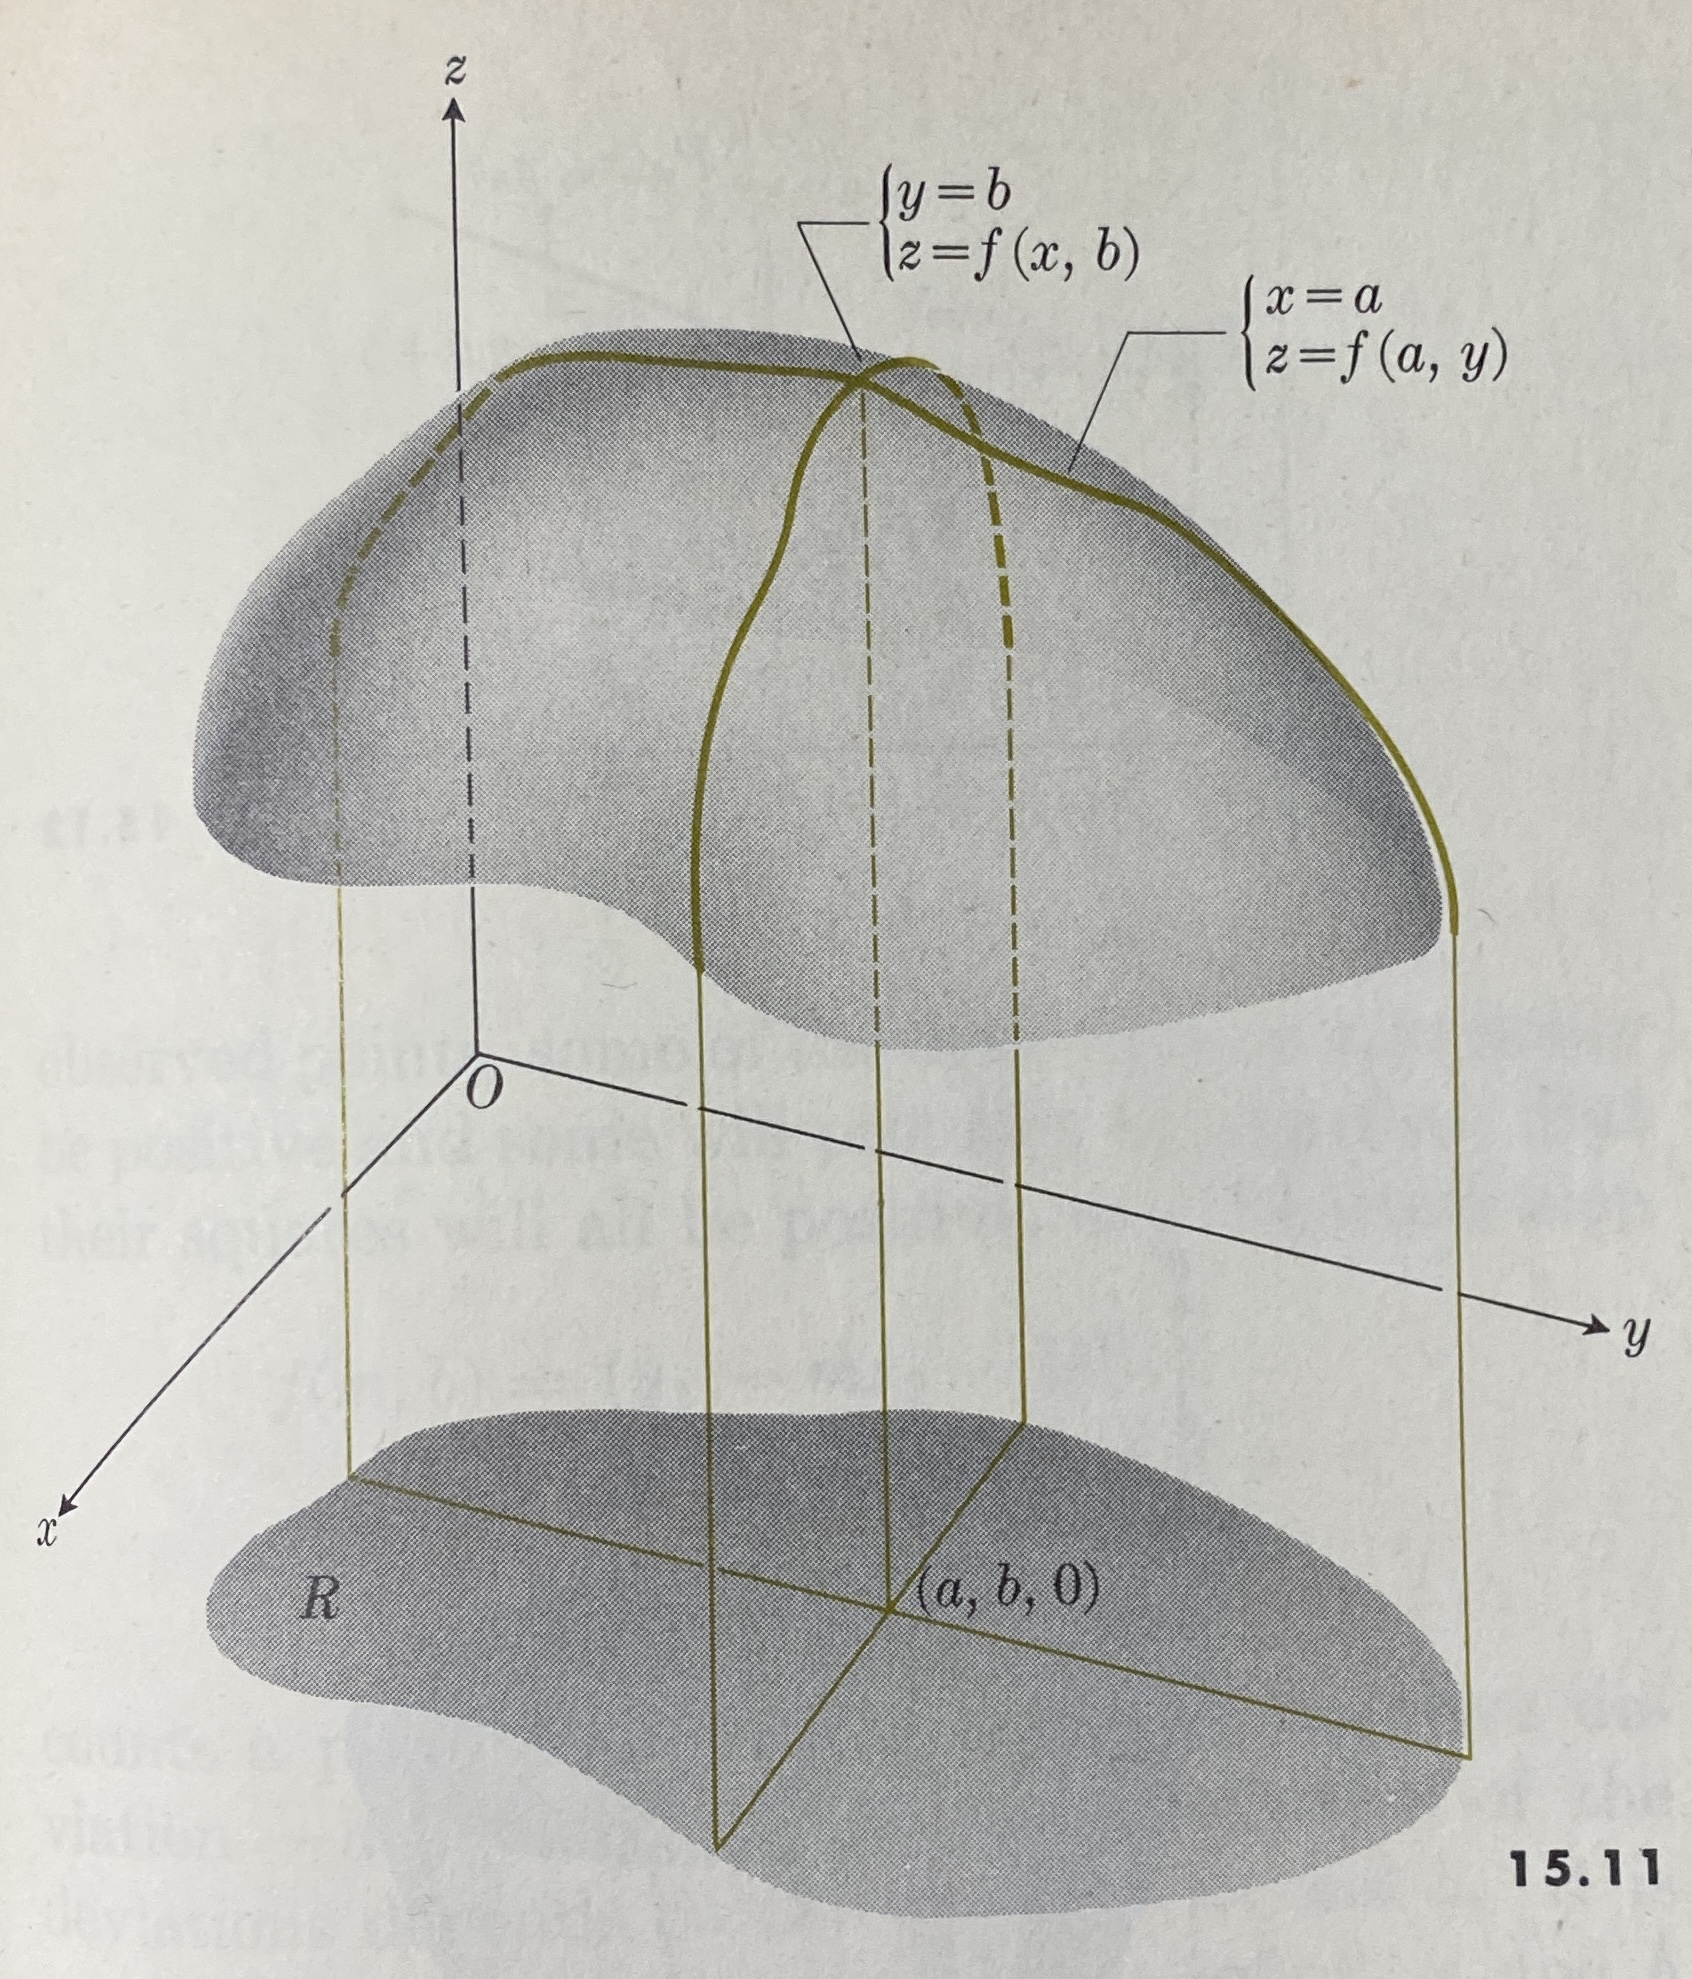
\includegraphics[width=0.4\linewidth]{ExtFiles/relativeMaximum.jpg}
        \caption{Relative maximum of $f(x,y)$.}
        \label{fig:relativeMaximum}
    \end{figure}
    \item If $(a,b)$ is a relative maximum\footnote{Or minimum. We choose arbitrarily to work with maxima from here on out, but every statement is symmetric for minima.}, then $f_x(a,b)=0$ and $f_y(a,b)=0$.
    \begin{itemize}
        \item We can see from Figure \ref{fig:relativeMaximum} that the curve lying in the plane $y=b$ given by $z=f(x,b)$ has a high turning point at $x=a$.
        \item We can similarly see that $z=f(a,y)$ has a high turning point at $y=b$.
        \item Thus,
        \begin{align*}
            \left( \pdv{z}{x} \right)_{(a,b)} &= 0&
                \left( \pdv{z}{y} \right)_{(a,b)} &= 0
        \end{align*}
        \item This implies the desired result.
    \end{itemize}
    \item As to the second derivative test, \cite{bib:Thomas} does not go into it deeply, but mentions that the key is that $D=f(x,y)-f(a,b)$ is nonnegative (positive or zero) for a minimum and nonpositive (negative or zero) for a maximum for all $(x,y)$ sufficiently close to $(a,b)$.
    \begin{itemize}
        \item He recommends checking $x=a+h$ and $y=b+k$ for small values of $h$ and $k$ to confirm.
        \item This may seem to not be rigorous, but it can actually work quite well, as we will see in the following problem.
    \end{itemize}
    \item Find the minima and maxima on the surface
    \begin{equation*}
        z = f(x,y) = x^2-xy+y^2+2x+2y-4
    \end{equation*}
    \begin{itemize}
        \item Since the domain of this functions is not restricted, there are no boundary points to check. Thus, we need only apply the necessary conditions
        \begin{align*}
            0 &= \pdv{z}{x}&
                0 &= \pdv{z}{y}\\
            &= 2x-y+2&
                &= 2y-x+2
        \end{align*}
        \item If we solve the above as a two-variable system of equations, we find that $(-2,-2)$ is the solution.
        \item Thus, the critical point is $(-2,-2,f(-2,-2))=(-2,-2,-8)$.
        \item Applying the pseudo-second-derivative test, we have
        \begin{align*}
            D &= f(-2+h,-2+k)-f(-2,-2)\\
            &= h^2-hk+k^2\\
            &= \left( h-\frac{k}{2} \right)^2+\frac{3k^2}{4}
        \end{align*}
        which is clearly positive unless $h=k=0$.
        \item Therefore, $(-2,-2,-8)$ is an absolute minimum, and there are no other high or low points.
    \end{itemize}
\end{itemize}



\section{The Method of Least Squares}
\begin{figure}[H]
    \centering
    \begin{subfigure}[b]{0.4\linewidth}
        \centering
        \begin{tikzpicture}[
            every node/.style={black}
        ]
            \footnotesize
            \draw [->] (-0.6,0) -- (5,0) node[right]{$x$};
            \draw [->] (0,-0.6) -- (0,3.5) node[above]{$y$};
            \node [anchor=north east] {$O$};

            \draw [ylx,thick] (0.1,1) -- node[pos=0.7,right,yshift=-1mm]{$y=mx+b$} (4.5,3);
            \node (P1) [circle,fill,inner sep=1.5pt,ylx,label={[xshift=3mm]above:$P_1(x_1,y_1)$}] at (0.5,1.8) {}
                (P1.center) edge [ylx,semithick] (0.5,1.18);
            ;
            \node (P2) [circle,fill,inner sep=1.5pt,ylx,label={right:$P_2(x_2,y_2)$}] at (1.5,1.15) {}
                (P2.center) edge [ylx,semithick] (1.5,1.64);
            ;
            \node (P) [circle,fill,inner sep=1.5pt,ylx] at (2.5,1.75) {}
                (P.center) edge [ylx,semithick] (2.5,2.09);
            ;
            \node (Pn) [circle,fill,inner sep=1.5pt,ylx,label={above:$P_n(x_n,y_n)$}] at (3.5,2.8) {}
                (Pn.center) edge [ylx,semithick] (3.5,2.55);
            ;
        \end{tikzpicture}
        \caption{Best fit line.}
        \label{fig:leastSquaresa}
    \end{subfigure}
    \begin{subfigure}[b]{0.4\linewidth}
        \centering
        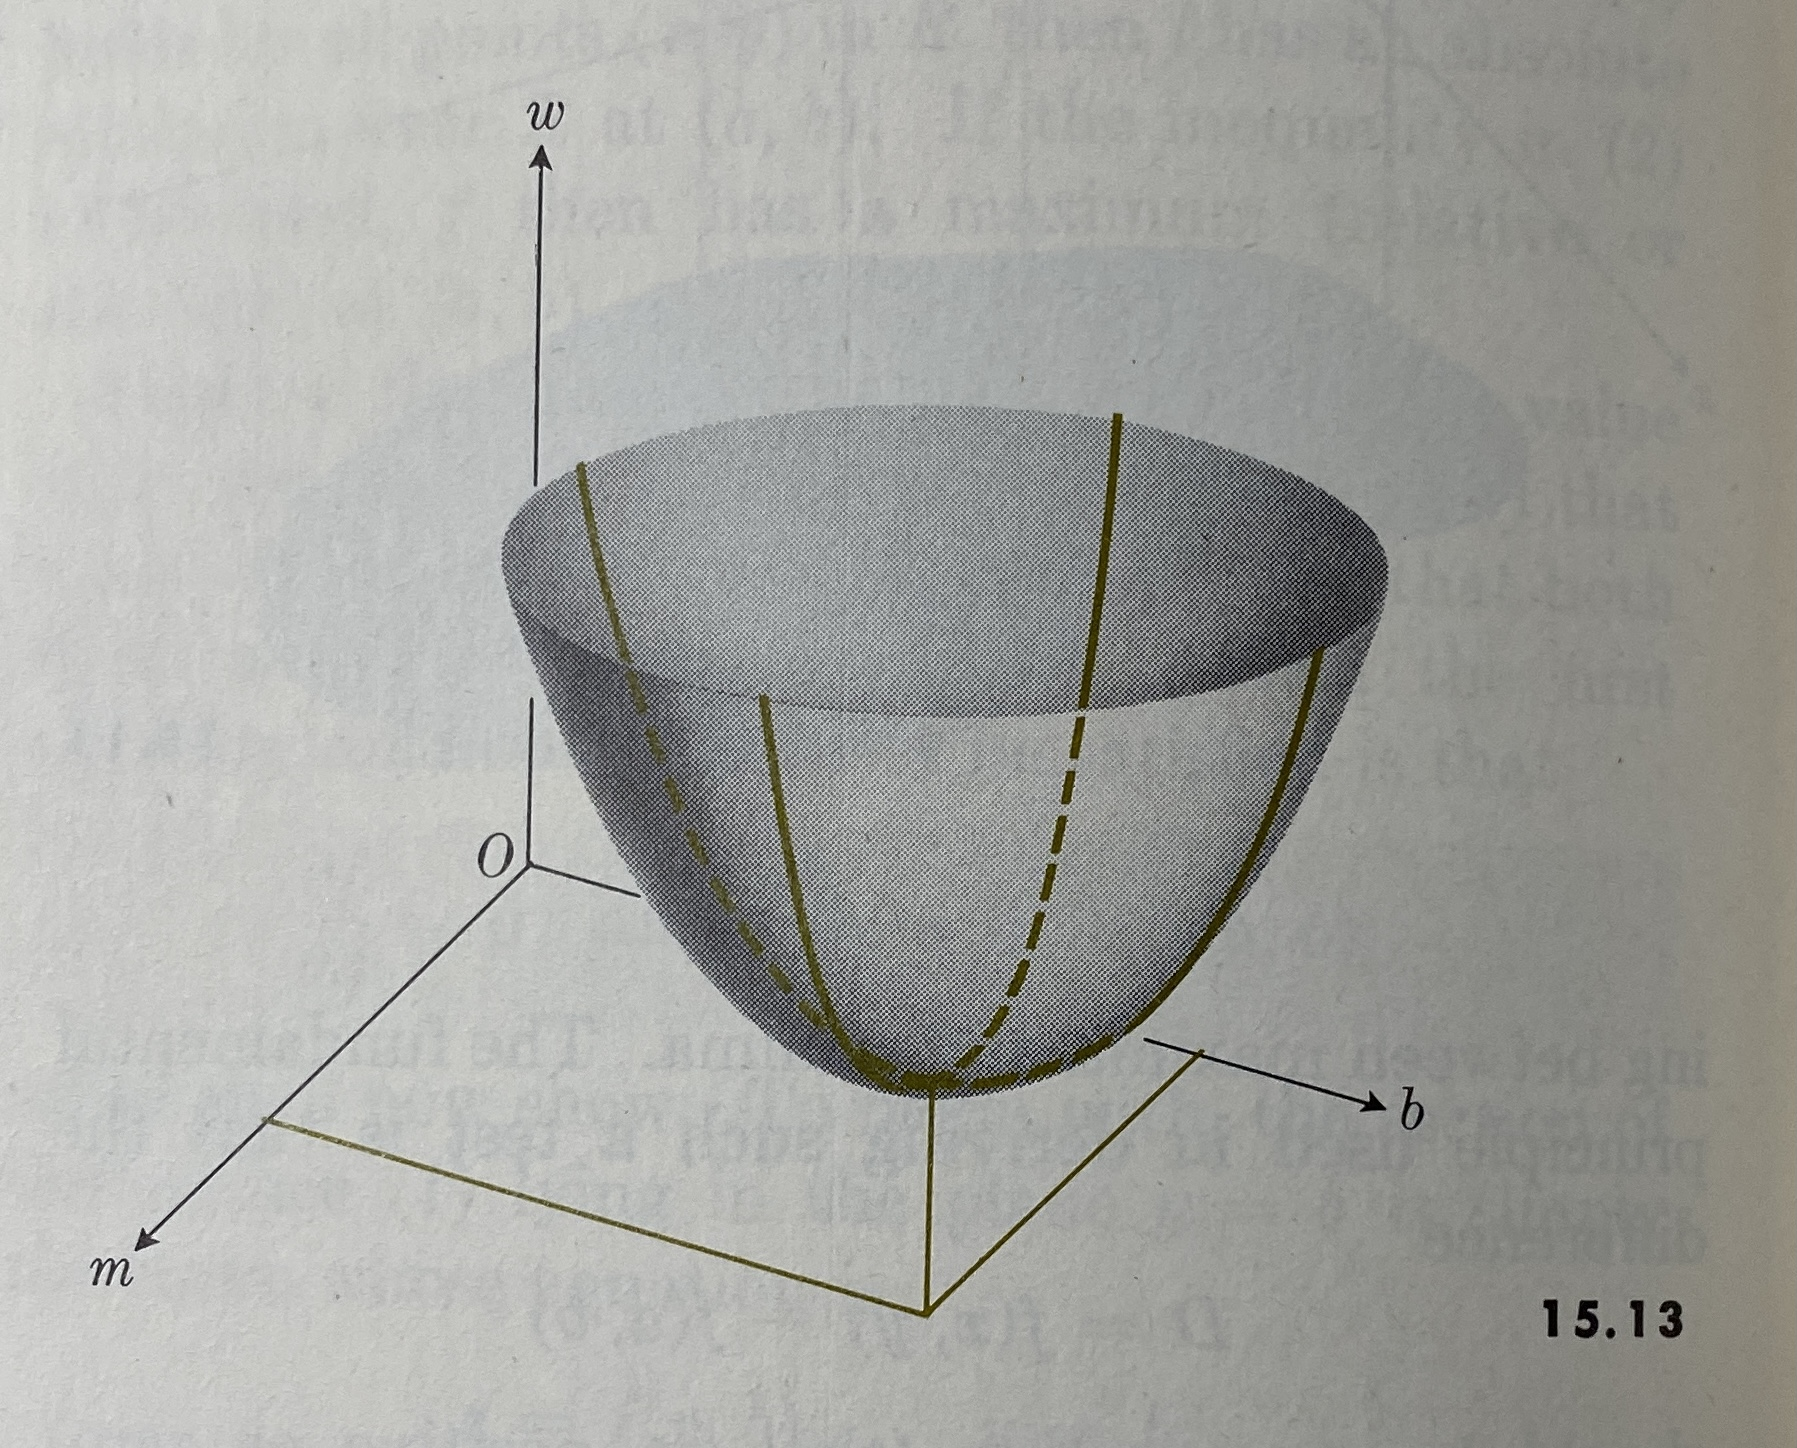
\includegraphics[width=0.9\linewidth]{ExtFiles/leastSquaresb.jpg}
        \caption{Minimization.}
        \label{fig:leastSquaresb}
    \end{subfigure}
    \caption{Method of least squares.}
    \label{fig:leastSquares}
\end{figure}
\begin{itemize}
    \item \textbf{Method of least squares}: A technique for fitting a straight line $y=mx+b$ to a set of experimentally observed points $(x_1,y_1),(x_2,y_2),\dots,(x_n,y_n)$.
    \item \textbf{Deviation}: The difference between the observed $y$-value and the $y$-value predicted by the straight line. \emph{Also known as} \textbf{dev}, $\bm{d_n}$.
    \begin{equation*}
        \text{dev} = y_\text{obs}-(mx_\text{obs}+b)
    \end{equation*}
    \item \dq{For a straight line which comes close to fitting all of the observed points, some of the deviations will probably be positive and some will probably be negative. But their squares will all be positive, and the expression $$f(m,b)=(y_1-mx_1-b)^2+(y_2-mx_2-b)^2+\cdots+(y_n-mx_n-b)^2$$ counts a positive deviation $+d$ and a negative deviation $-d$ equally. This sum of squares of the deviations depends on the choice of $m$ and $b$. It is never negative, and it can be zero only if $m$ and $b$ have values that produce a straight line that is a perfect fit}{524-25}
    \begin{itemize}
        \item Essentially, the method of least squares says \dq{Take as the line $y=mx+b$ of best fit that one for which the sum of squares of the deviations $$f(m,b)=d_1^2+d_2^2+\cdots+d_n^2$$ is a minimum}{525}
    \end{itemize}
    \item Note that we can use the pseudo-second-derivative test to show that the point on $f(m,b)$ found by the method of least squares is a minimum. However, it is customary to omit this step since it can be shown that for the general case of fitting a straight line, the answer is always a minimum.
\end{itemize}



\section{Maxima and Minima of Functions of Several Independent Variables}
\begin{itemize}
    \item This is necessary in certain statistical applications.
    \item As we would expect, minima and maxima of functions of the form $w=f(x_1,\dots,x_n)$ can lie at boundary points, or at points where $0=\pdv*{f}{x_1},\dots,\pdv*{f}{x_n}$.
    \item Sometimes a function $w=f(x_1,\dots,x_n)$ is given with certain constraints of the form $g(x_1,\dots,x_n)=0$. In these cases, use the constraints to express some of the variables in terms of the remaining ones (so that the remaining ones are independent) before taking partial derivatives.
    \item The minimization process may lead to an answer that lies outside the region where $f$ is defined. In these cases, it can help to choose a different set of independent variables. Let's look at one example of this phenomenon.
    \item \dq{Find the minimum distance from the origin to the surface $x^2-z^2=1$}{528}
    \begin{figure}[h!]
        \centering
        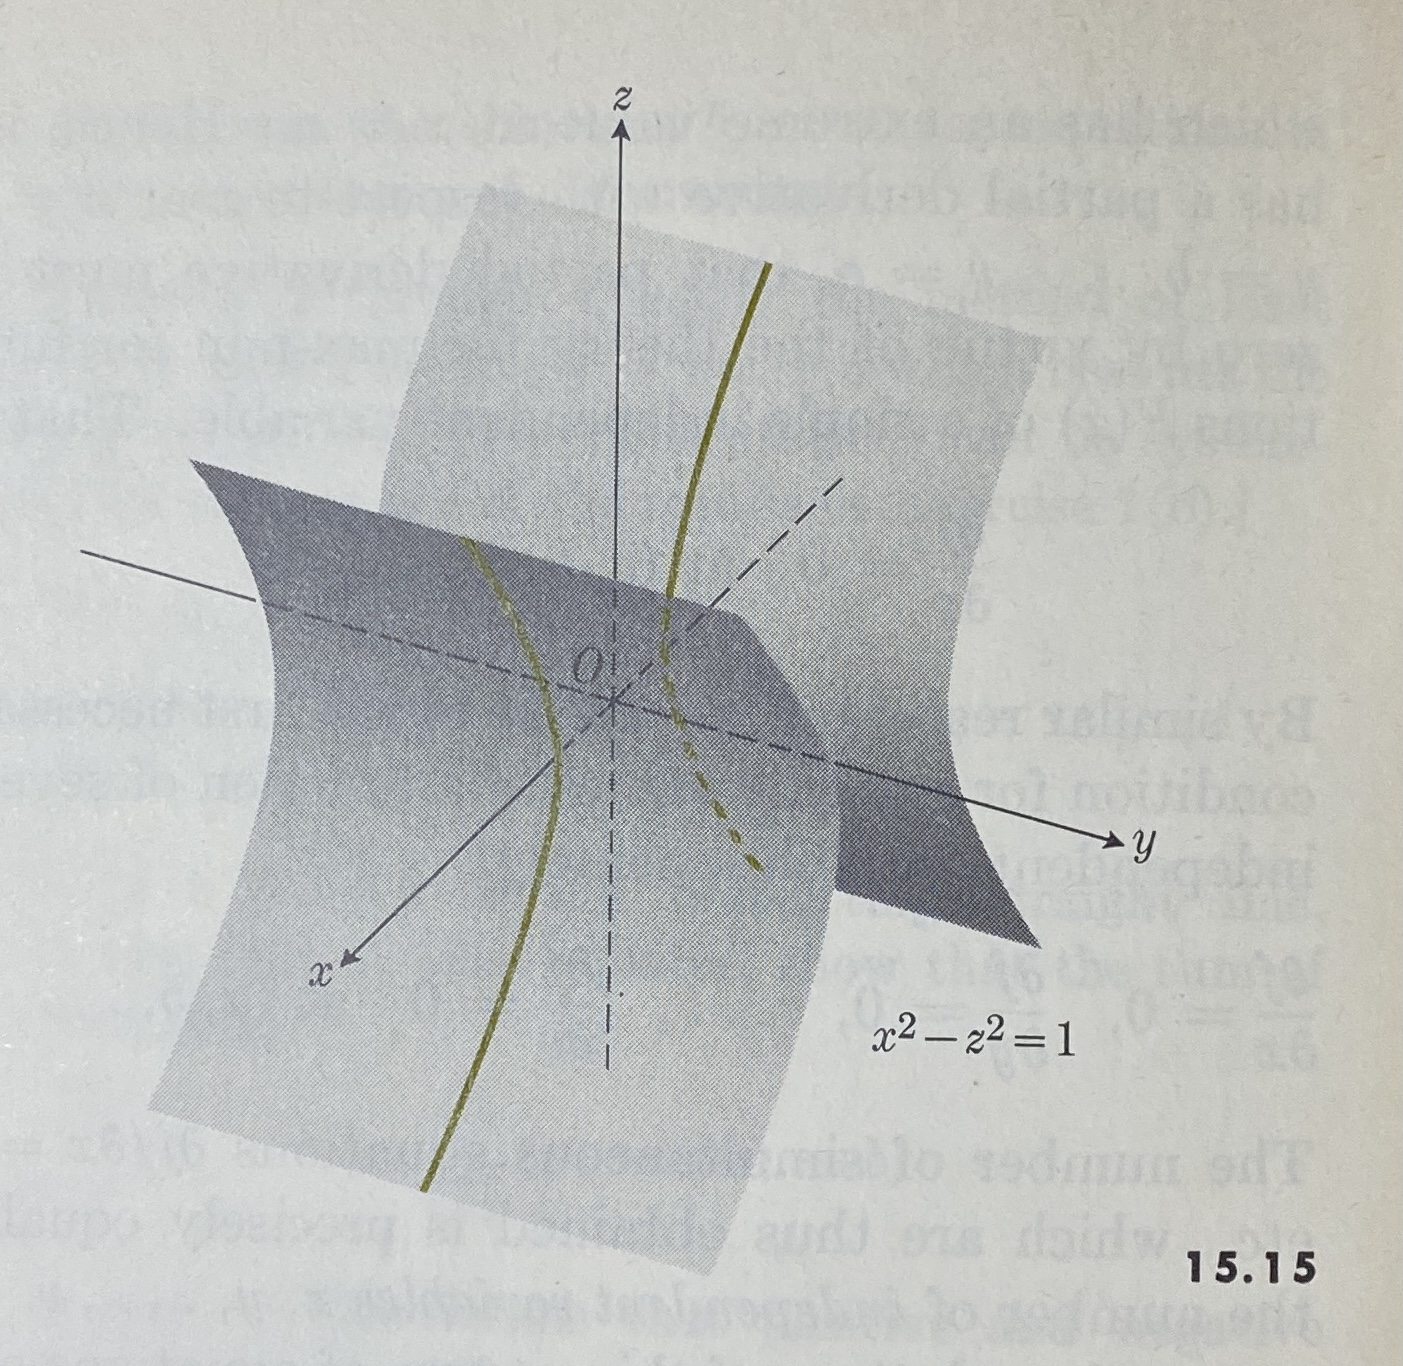
\includegraphics[width=0.4\linewidth]{ExtFiles/minimizeHyperbolicCylinder.jpg}
        \caption{Minimizing the distance from the origin across a hyperbolic cylinder.}
        \label{fig:minimizeHyperbolicCylinder}
    \end{figure}
    \begin{itemize}
        \item We want to minimize $\sqrt{(x-0)^2+(y-0)^2+(z-0)^2}$, the formula for the distance between a point $(x,y,z)$ and the origin, over all points $(x,y,z)$ on the surface defined by $x^2-z^2=1$.
        \item Thus, we choose to minimize $w=x^2+y^2+z^2$ (it's easier to work without the radical, and the latter formula minimizes at the same points as the former). To limit the set of points in the domain of $w$, we arbitrarily choose $x$ and $y$ to be our independent variables and use the constraint to substitute out $z$, yielding $w=2x^2+y^2-1$.
        \item However, $0=\pdv*{w}{x}=4x$ and $0=\pdv*{w}{y}=2y$ lead to $(0,0,i)$ as our answer. The problem here is that $x\in(-1,1)$ is not in the domain of $x^2-z^2=1$, yet it is in the domain of $w=2x^2+y^2-1$.
        \item Thus, we need a different substitution. If we eliminate $x$ instead, then we have $w=1+y^2+2z^2$ in terms of variables that have meaning for all values in the set $(-\infty,\infty)$ (importantly, no new elements are added to the domain). Indeed, minimizing this, we get $(\pm 1,0,0)$ as our answers, and we can see from Figure \ref{fig:minimizeHyperbolicCylinder} that these are correct.
    \end{itemize}
    \item \textbf{Method of Lagrange multipliers}: \dq{To minimize (or maximize) a function $f(x,y,z)$, subject to the constraint $g(x,y,z)=0$, construct the auxiliary function $$H(x,y,z,\lambda)=f(x,y,z)-\lambda g(x,y,z)$$ and find values of $x,y,z,\lambda$ for which the partial derivatives of $H$ are all 0: $H_x=0$, $H_y=0$, $H_z=0$, [and] $H_\lambda=0$}{528}
    \item \dq{Find the point on the plane $$2x-3y+5z=19$$ that is nearest the origin, using the method of Lagrange multipliers}{528}
    \begin{itemize}
        \item Find $H$.
        \begin{equation*}
            H(x,y,z,\lambda) = x^2+y^2+z^2-\lambda(2x-3y+5z-19)
        \end{equation*}
        \item Take partial derivatives.
        \begin{align*}
            0 &= H_x = 2x-2\lambda&
                0 &= H_y = 2y+3\lambda&
                    0 &= H_z = 2z-5\lambda&
                        0 &= H_\lambda = -g(x,y,z)
        \end{align*}
        \item Solve $H_x,H_y,H_z$ for $x,y,z$.
        \begin{align*}
            x &= \lambda&
                y &= -\frac{3}{2}\lambda&
                    z &= \frac{5}{2}\lambda
        \end{align*}
        \item Plug into $H_\lambda$ and solve for $\lambda$.
        \begin{align*}
            2\lambda+\frac{9}{2}\lambda+\frac{25}{2}\lambda &= 19\\
            \lambda &= 1
        \end{align*}
        \item Return the substitutions.
        \begin{equation*}
            (x,y,z) = \left( 1,-\frac{3}{2},\frac{5}{2} \right)
        \end{equation*}
    \end{itemize}
    \item \cite{bib:Thomas} derives the method of Lagrange multiplies, finding in the process the important equation $\nabla f=\lambda\nabla g$ where $\lambda=f_z/g_z$\footnote{There is some important but rather indecipherable geometric meaning of this equation. Additionally, the proof overall would be good to understand. This is something to come back to at a later date, though.}.
    \item If there exist two constraints $g(x,y,z)$ and $h(x,y,z)$, then we work with
    \begin{equation*}
        H(x,y,z,\lambda,\mu) = f(x,y,z)-\lambda g(x,y,z)-\mu h(x,y,z)
    \end{equation*}
    and set $H_x,H_y,H_z,H_\lambda,H_\mu=0$ in the process.
    \begin{itemize}
        \item We also have in this case $\nabla f=\lambda\nabla g+\mu\nabla h$.
    \end{itemize}
\end{itemize}



\section{Higher-Order Derivatives}
\begin{itemize}
    \item \marginnote{12/19:}To denote higher-order partial derivatives, use symbols such as
    \begin{equation*}
        \pdv[2]{f}{x},\ \pdv[2]{f}{y},\ \pdv{f}{x}{y},\ \pdv{f}{y}{x}
    \end{equation*}
    or, respectively,
    \begin{equation*}
        f_{xx},\ f_{yy},\ f_{yx},\ f_{xy}
    \end{equation*}
    \item The order of differentiation is "conserved" left to right, in a sense. For example,
    \begin{equation*}
        \pdv{f}{x}{y} = \pdv{x}\left( \pdv{f}{y} \right)
    \end{equation*}
    \item However, in general, $\pdv*{f}{x}{y}=\pdv*{f}{y}{x}$:
    \begin{thm}\label{thm:pdvOrdering}
        Let the function $w=f(x,y)$, together with the partial derivatives $f_x$, $f_y$, $f_{xy}$, and $f_{yx}$ be continuous in some neighborhood of a point $P(a,b)$. Then, at that point,
        \begin{equation*}
            \pdv{x}\left( \pdv{f}{y} \right) = \pdv{y}\left( \pdv{f}{x} \right)
        \end{equation*}
        \begin{figure}[h!]
            \centering
            \begin{tikzpicture}[
                every node/.append style={black}
            ]
                \footnotesize
                \draw [->] (-0.6,0) -- (5,0) node[right]{$x$};
                \draw [->] (0,-0.6) -- (0,3.5) node[above]{$y$};
                \node [anchor=north east] {$O$};

                \fill [yly!60] (0.8,0.6) rectangle (4.2,2.8) node[below right]{$R$};
                \fill [yly] (1.6,1.3) node[circle,fill,inner sep=1.5pt,label={[xshift=-2mm]below:$(a,b)$}]{} -- node[below]{$h$} (3.6,1.3) -- node[pos=0.6,right]{$R'$} (3.6,2.4) -- (1.6,2.4) -- node[left]{$k$} cycle;
            \end{tikzpicture}
            \caption{Equivalence of higher-order partial derivative ordering.}
            \label{fig:pdvOrdering}
        \end{figure}
        \begin{proof}
            Let $h$ and $k$ be numbers such that $(a+h,b+k)$ lies in the rectangle $R$, and let $F(x)$ be defined by $F(x)=f(x,b+k)-f(x,b)$. Consider the difference
            \begin{equation*}
                \Delta = F(a+h)-F(a)
            \end{equation*}
            If we apply the Mean Value Theorem to $F$, we get
            \begin{equation*}
                \Delta = hF'(c_1)
            \end{equation*}
            for some $c_1\in[a,a+h]$. Substituting, we have
            \begin{equation*}
                \Delta = h[f_x(c_1,b+k)-f_x(c_1,b)]
            \end{equation*}
            If we apply the Mean Value Theorem to the difference $f_x(c_1,b+k)-f_x(c_1,b)$, we get $f_x(c_1,b+k)-f_x(c_1,b)=kf_{xy}(c_1,d_1)$ where $d_1\in[b,b+k]$. Therefore,
            \begin{equation*}
                \Delta = hkf_{xy}(c_1,d_1)
            \end{equation*}
            where $(c_1,d_1)\in R'$ in Figure \ref{fig:pdvOrdering}. Now, if we let $G(y)=f(a+h,y)-f(a,y)$, we can arrive at the similar result
            \begin{equation*}
                \Delta = hkf_{yx}(c_2,d_2)
            \end{equation*}
            where $(c_2,d_2)\in R'$ in Figure \ref{fig:pdvOrdering}. Thus, by transitivity, we have
            \begin{equation*}
                f_{xy}(c_1,d_1) = f_{yx}(c_2,d_2)
            \end{equation*}
            That is not what we wanted to prove. However, since $h$ and $k$ can be made arbitrarily small, and since the continuity of $f_{xy}$ and $f_{yx}$ implies that
            \begin{align*}
                f_{xy}(c_1,d_1) &= f_{xy}(a,b)+\epsilon_1&
                    f_{yx}(c_2,d_2) &= f_{yx}(a,b)+\epsilon_2
            \end{align*}
            where $\epsilon_1,\epsilon_2\to 0$ as $h,k\to 0$, we let $h,k\to 0$ and get
            \begin{equation*}
                f_{xy}(a,b) = f_{yx}(a,b)
            \end{equation*}
            as desired.
        \end{proof}
    \end{thm}
    \item Note that the quantity $\Delta$ in the above proof of Theorem \ref{thm:pdvOrdering} is known as the \textbf{second difference}.
    \begin{itemize}
        \item Although it is an advanced skill to know introduce such a tool in a proof, it makes sense to use the \emph{second} difference in a proof about \emph{second} derivatives.
        \item Note that for sufficiently small $h,k$, $\Delta\approx hkf_{xy}(a,b)$.
    \end{itemize}
    \item From Theorem \ref{thm:pdvOrdering}, we can prove higher-order partial derivative equalities such as
    \begin{equation*}
        \frac{\partial^3f}{\partial x^2\partial y} = \pdv{x}\left( \pdv{f}{x}{y} \right)
        = \pdv{x}\left( \pdv{f}{y}{x} \right)
        = \pdv{y}\left( \pdv{f}{x}{x} \right)
        = \frac{\partial^3f}{\partial y\partial x^2}
    \end{equation*}
    \item \dq{In fact, if all the partial derivatives that appear are continuous, the notation $$\frac{\partial^{m+n}f}{\partial x^m\partial y^n}$$ may be used to denote the result of differentiating the function $f(x,y)$ $m$ times with respect to $x$ and $n$ times with respect to $y$, the order in which these differentiations are performed being entirely arbitrary}{535}
\end{itemize}



\section{Exact Differentials}
\begin{itemize}
    \item \textbf{Exact differential}: The expression $\dd{f(x,y)}=M(x,y)\dd{x}+N(x,y)\dd{y}$ corresponding to a function $w=f(x,y)$.
    \begin{figure}[h!]
        \centering
        \begin{subfigure}[b]{0.4\linewidth}
            \centering
            \begin{tikzpicture}
                \fill [yly] plot[smooth cycle] coordinates{(0,0) (0.3,0.1) (0.5,0.4) (0.9,0.7) (1,1) (0.9,1.3) (0.5,1.5) (-0.4,1.6) (-1,1.7) (-1.4,1.5) (-1.5,1.2) (-1.1,0.8) (-0.6,0.3)};
            \end{tikzpicture}
            \caption{A simply connected region.}
            \label{fig:regionsa}
        \end{subfigure}
        \begin{subfigure}[b]{0.4\linewidth}
            \centering
            \begin{tikzpicture}
                \fill [yly] (0,0)
                    to[out=0,in=-90] (1,1)
                    to[out=90,in=0] (0.3,1.7)
                    to[out=180,in=0] (-0.5,1.5)
                    to[out=180,in=90,in looseness=0.7] (-1.8,0.8)
                    to[out=-90,in=180,out looseness=0.7] cycle
                ;
                \fill [white] (0.3,0.9)
                    to[out=0,in=-90,out looseness=1.2] (0.5,1.1)
                    to[out=90,in=0] (0.2,1.3)
                    to[out=180,in=90] (0,1.1)
                    to[out=-90,in=180] cycle
                ;
                \fill [white] (-0.6,0.7)
                    to[out=0,in=-90,out looseness=0.7,in looseness=0.8] (-0.2,1.1)
                    to[out=90,in=0] (-0.4,1.3)
                    to[out=180,in=90,out looseness=0.8,in looseness=0.7] (-0.8,0.9)
                    to[out=-90,in=180] cycle
                ;
                \fill [white] (0,0.2)
                    to[out=0,in=-90] (0.2,0.4)
                    to[out=90,in=0,in looseness=0.6] (0,0.6)
                    to[out=180,in=45,out looseness=0.6] (-0.2,0.5)
                    to[out=-135,in=90] (-0.4,0.3)
                    to[out=-90,in=180,out looseness=0.6] cycle
                ;
            \end{tikzpicture}
            \caption{A (not simply) connected region.}
            \label{fig:regionsb}
        \end{subfigure}\\
        \vspace{1em}
        \begin{subfigure}[b]{0.4\linewidth}
            \centering
            \begin{tikzpicture}
                \fill [yly] (0,0)
                    -- (1,0.2)
                    to[out=100,in=0] (-0.3,1.3)
                    to[out=180,in=90] (-2,-0.2)
                    to[out=-90,in=180] (-1.5,-1)
                    to[out=0,in=180] (-0.8,-0.9)
                    to[out=0,in=180] (0,-1)
                    to[out=0,in=-60,in looseness=1.2] (0.4,-0.1)
                    -- (-0.2,-0.15)
                    to [out=-100,in=0] (-0.7,-0.4)
                    to[out=180,in=-90] (-1.1,-0.1)
                    to[out=90,in=180] (-0.6,0.4)
                    to[out=0,in=110] cycle
                ;
            \end{tikzpicture}
            \caption{A simply connected region.}
            \label{fig:regionsc}
        \end{subfigure}
        \begin{subfigure}[b]{0.4\linewidth}
            \centering
            \begin{tikzpicture}
                \footnotesize
                \fill [yly] (0,1.5)
                    to[out=-90,in=180] (0.7,0.8)
                    to[out=0,in=-90,in looseness=0.7] (2,1.7)
                    to[out=90,in=0,out looseness=0.8,in looseness=1.2] (1.2,2.2)
                    to[out=180,in=90,in looseness=0.9] cycle
                ;
                \fill [yly] (2,0)
                    to[out=0,in=-90] (3.3,1)
                    to[out=90,in=0] (2.7,1.5)
                    to[out=180,in=90,out looseness=0.7,in looseness=0.8] (1.5,0.5)
                    to[out=-90,in=180] cycle
                ;
                \fill (0.6,1.6) circle (1.5pt) node[right]{$A$};
                \fill (2.1,0.7) circle (1.5pt) node[right]{$B$};
            \end{tikzpicture}
            \caption{A disconnected region (no path $AB$ lies entirely within the set, for example).}
            \label{fig:regionsd}
        \end{subfigure}
        \caption{Types of regions in the plane.}
        \label{fig:regions}
    \end{figure}
    \item \textbf{Simply connected region} (of the plane): A set of points that is \textbf{open}, \textbf{connected}, and satisfies the property that \dq{if $C$ is any simple closed curve, all of whose points are in the set, then all points in the interior of $C$ are also in the set}{537}
    \item \textbf{Open} (set in the plane): A set such that \dq{each point of the set is an \textbf{interior} point of the set}{537}
    \item \textbf{Connected} (set): A set such that \dq{any two points of the set can be joined by a polygonal path, all of whose points are in the set}{537}
    \item \textbf{Interior} (point of a set in the plane): A point that \dq{can be the center of a small circle whose entire interior is in the set}{537}
    \item We now prove a theorem that answers two questions with respect to exact differentials: (1) "How can we tell whether a given expression is or is not an exact differential?" and (2) \dq{If the expression is exact, how do we find the function $f(x,y)$ of which it is the differential?}{536}
    \begin{thm}\label{thm:exactDifferential}
        Let the functions $M(x,y)$ and $N(x,y)$ be continuous, and let them possess continuous partial derivatives $M_x,M_y,N_x,N_y$ for all real values of $x$ and $y$ in some simply connected region $G$. Then a necessary and sufficient condition for $M(x,y)\dd{x}+N(x,y)\dd{y}$ to be an exact differential in $G$ is that
        \begin{equation*}
            \pdv{M}{y} = \pdv{N}{x}
        \end{equation*}
        \begin{proof}
            We first demonstrate that $\pdv*{M}{y}=\pdv*{N}{x}$ is a necessary condition. Suppose that there exists a function $f(x,y)$ with an exact differential at all points in $G$. We also know that $\dd{f}=\pdv*{f}{x}\dd{x}+\pdv*{f}{y}\dd{y}$ by the definition of the total differential. Thus,
            \begin{equation*}
                M(x,y)\dd{x}+N(x,y)\dd{y} = \pdv{f}{x}\dd{x}+\pdv{f}{y}\dd{y}
            \end{equation*}
            But since $\dd{x}$ and $\dd{y}$ are independent variables in the above equation, we can set either to 0 and the equality must be maintained. Consequently, we must have
            \begin{align*}
                \pdv{f}{x} &= M(x,y)&
                    \pdv{f}{y} &= N(x,y)
            \end{align*}
            Now by Theorem \ref{thm:pdvOrdering}, we have
            \begin{equation*}
                \pdv{y}\left( \pdv{f}{x} \right) = \pdv{x}\left( \pdv{f}{y} \right)
            \end{equation*}
            and it follows from this that
            \begin{equation*}
                \pdv{M}{y} = \pdv{N}{x}
            \end{equation*}
            as desired.\par
            To demonstrate that $\pdv*{M}{y}=\pdv*{N}{x}$ is a sufficient condition, we will show how to find the function $f(x,y)$ from the exact differential. To begin, let $\pdv*{f}{x}=M(x,y)$. From this definition, the condition that $\pdv*{M}{y}=\pdv*{N}{x}$, and Theorem \ref{thm:pdvOrdering}, we can immediately learn another interesting fact about $f$:
            \begin{align*}
                \pdv{y}\left( \pdv{f}{x} \right) &= \pdv{M}{y}\\
                \pdv{x}\left( \pdv{f}{y} \right) &= \pdv{N}{x}\\
                \pdv{f}{y} &= N(x,y)
            \end{align*}
            With this established, we can now solve for $f(x,y)$. Start with
            \begin{align*}
                \pdv{f}{x} &= M(x,y)
                \intertext{From here, we integrate both sides with respect to $x$, holding $y$ constant. Notice that we introduce $g(y)$, a function of just $y$, as a kind of constant of integration\footnotemark.}
                f(x,y) &= \int_x M(x,y)\dd{x}+g(y)
                \intertext{We now take the partial derivative with respect to $y$.}
                \pdv{f}{y} &= \pdv{y}\int_x M(x,y)\dd{x}+\pdv{g}{y}
                \intertext{Since $g$ is purely a function of $y$, the partial derivative of $g$ with respect to $y$ is simply the derivative of $g$ with respect to $y$.}
                &= \pdv{y}\int_x M(x,y)\dd{x}+\dv{g}{y}
                \intertext{We now make use of the fact that we proved in the beginning, and substitute out $\pdv{f}{y}$ for $N(x,y)$. We then rearrange the terms to create a differential equation for $g$.}
                N(x,y) &= \pdv{y}\int_x M(x,y)\dd{x}+\dv{g}{y}\\
                \dv{g}{y} &= N(x,y)-\pdv{y}\int_x M(x,y)\dd{x}
            \end{align*}
            \footnotetext{In the sense that if we took the partial derivative of both sides of the following with respect to $x$, we would get the above.}
            This differential equation can be solved for $g$ by integrating the right-hand side with respect to $y$. After that has been accomplished, we can substitute the definition of $g$ back into $f(x,y)=\int_x M(x,y)\dd{x}+g(y)$ to generate the final formula for $f(x,y)$:
            \begin{equation*}
                f(x,y) = \int_x M(x,y)\dd{x}+\int_y\left( N(x,y)-\pdv{y}\int_x M(x,y)\dd{x} \right)\dd{y}
            \end{equation*}
        \end{proof}
    \end{thm}
    \item We now use an example to tangibly demonstrate both how to determine that a differential is a exact, and how to solve for $f(x,y)$.
    \item Consider the differential $(x^2+y^2)\dd{x}+2xy\dd{y}$. Use the condition of Theorem \ref{thm:exactDifferential} to show that it is exact, and then solve for the function $w=f(x,y)$ for which $\dd{w}=(x^2+y^2)\dd{x}+2xy\dd{y}$.
    \begin{itemize}
        \item Let $M(x,y)=x^2+y^2$ and let $N(x,y)=2xy$. Then
        \begin{equation*}
            \pdv{M}{y} = 2y = \pdv{N}{x}
        \end{equation*}
        so the given differential is exact.
        \item Now let $\pdv*{f}{x}=x^2+y^2$, and recall that we can prove from this that $\pdv*{f}{y}=2xy$. It follows that
        \begin{align*}
            f(x,y) &= \int_x(x^2+y^2)\dd{x}+g(y)\\
            &= \frac{x^3}{3}+xy^2+g(y)
            \intertext{The above equation is important, and we'll end up substituting $g(y)$ into it once we find it as follows.}
            \pdv{f}{y} &= \pdv{y}\left( \frac{x^3}{3}+xy^2 \right)+\pdv{g}{y}\\
            2xy &= 0+2xy+\dv{g}{y}\\
            \dv{g}{y} &= 0\\
            g(y) &= C\qquad C\in\R
        \end{align*}
        \item Therefore,
        \begin{equation*}
            f(x,y) = \frac{x^3}{3}+xy^2+C
        \end{equation*}
    \end{itemize}
\end{itemize}



\section{Derivatives of Integrals}
\begin{itemize}
    \item From the Fundamental Theorem of Integral Calculus, we know that if $f$ is a continuous function of $a\leq t\leq b$, then
    \begin{align*}
        \dv{x}\int_a^xf(t)\dd{t} &= f(x)&
            \dv{x}\int_x^bf(t)\dd{t} &= -f(x)
    \end{align*}
    \item These results allow us to prove the following.
    \begin{thm}
        Let $f$ be continuous on $a\leq t\leq b$. Let $u$ and $v$ be differentiable functions of $x$ such that $u(x)$ and $v(x)$ lie between $a$ and $b$. Then
        \begin{equation*}
            \dv{x}\int_{u(x)}^{v(x)}f(t)\dd{t} = f[v(x)]\dv{v}{x}-f[u(x)]\dv{u}{x}
        \end{equation*}
        \begin{proof}
            Let $F[u(x),v(x)]=\int_{u(x)}^{v(x)}f(t)\dd{t}$. Then by the above results from the Fundamental Theorem of Calculus, we respectively have
            \begin{align*}
                \pdv{F}{v} &= f[v(x)]&
                    \pdv{F}{u} &= -f[u(x)]
            \end{align*}
            Since $\dv*{F}{x}=\pdv*{F}{u}\dv*{u}{x}+\pdv*{F}{v}\dv*{v}{x}$ (the chain rule for partial derivatives), we therefore have
            \begin{align*}
                \dv{F}{x} &= -f[u(x)]\dv{u}{x}+f[v(x)]\dv{v}{x}\\
                \dv{x}\int_{u(x)}^{v(x)}f(t)\dd{t} &= f[v(x)]\dv{v}{x}-f[u(x)]\dv{u}{x}
            \end{align*}
            as desired.
        \end{proof}
    \end{thm}
\end{itemize}




\end{document}